\documentclass[
  final,
  babelLanguage=british,
  desktopVersion,
  %showtrims,
  %overleaf,
]{anecdote}

\graphicspath{{./assets/photos/300dpi/}}
%\graphicspath{{./assets/photos/92dpi/}}

% Blurb page size: 5 x 8 inch (127 x 203.2 mm)
% Body text: 10.5 / 16 pt

% Pocket page size: 135 x 120 mm
% Body text: 10.5 / 14 pt

\usepackage{local}

%% Details of the book
%% ===================

\title{Wordless Questioning}
\subtitle{an introduction to Buddhist meditation and reflection}
\author{Gambhīro Bhikkhu}
\publisher{The Publisher}% TODO
\date{2021-10-22}
\editionInfo{\textit{First edition}, 2021}% TODO update edition info
\ISBN{000-000-0000-00-0}% TODO update ISBN

% === Metadata ===

\hypersetup{
  pdftitle={\thetitle},
  pdfauthor={\theauthor},
  pdfcopyright={Copyright (C) 2021, \thePublisher},
  pdfsubject={},% TODO subject
  pdfkeywords={},% TODO keywords
  pdflicenseurl={https://creativecommons.org/licenses/by-nc-nd/4.0/},
  pdfcontacturl={},
  pdflang={en},
}

%% === Load further packages ===

%% === Hyphenation exceptions and corrections ===

\hyphenation{London}

\begin{document}

\frontmatter

\ifdesktopversion
\desktopCover{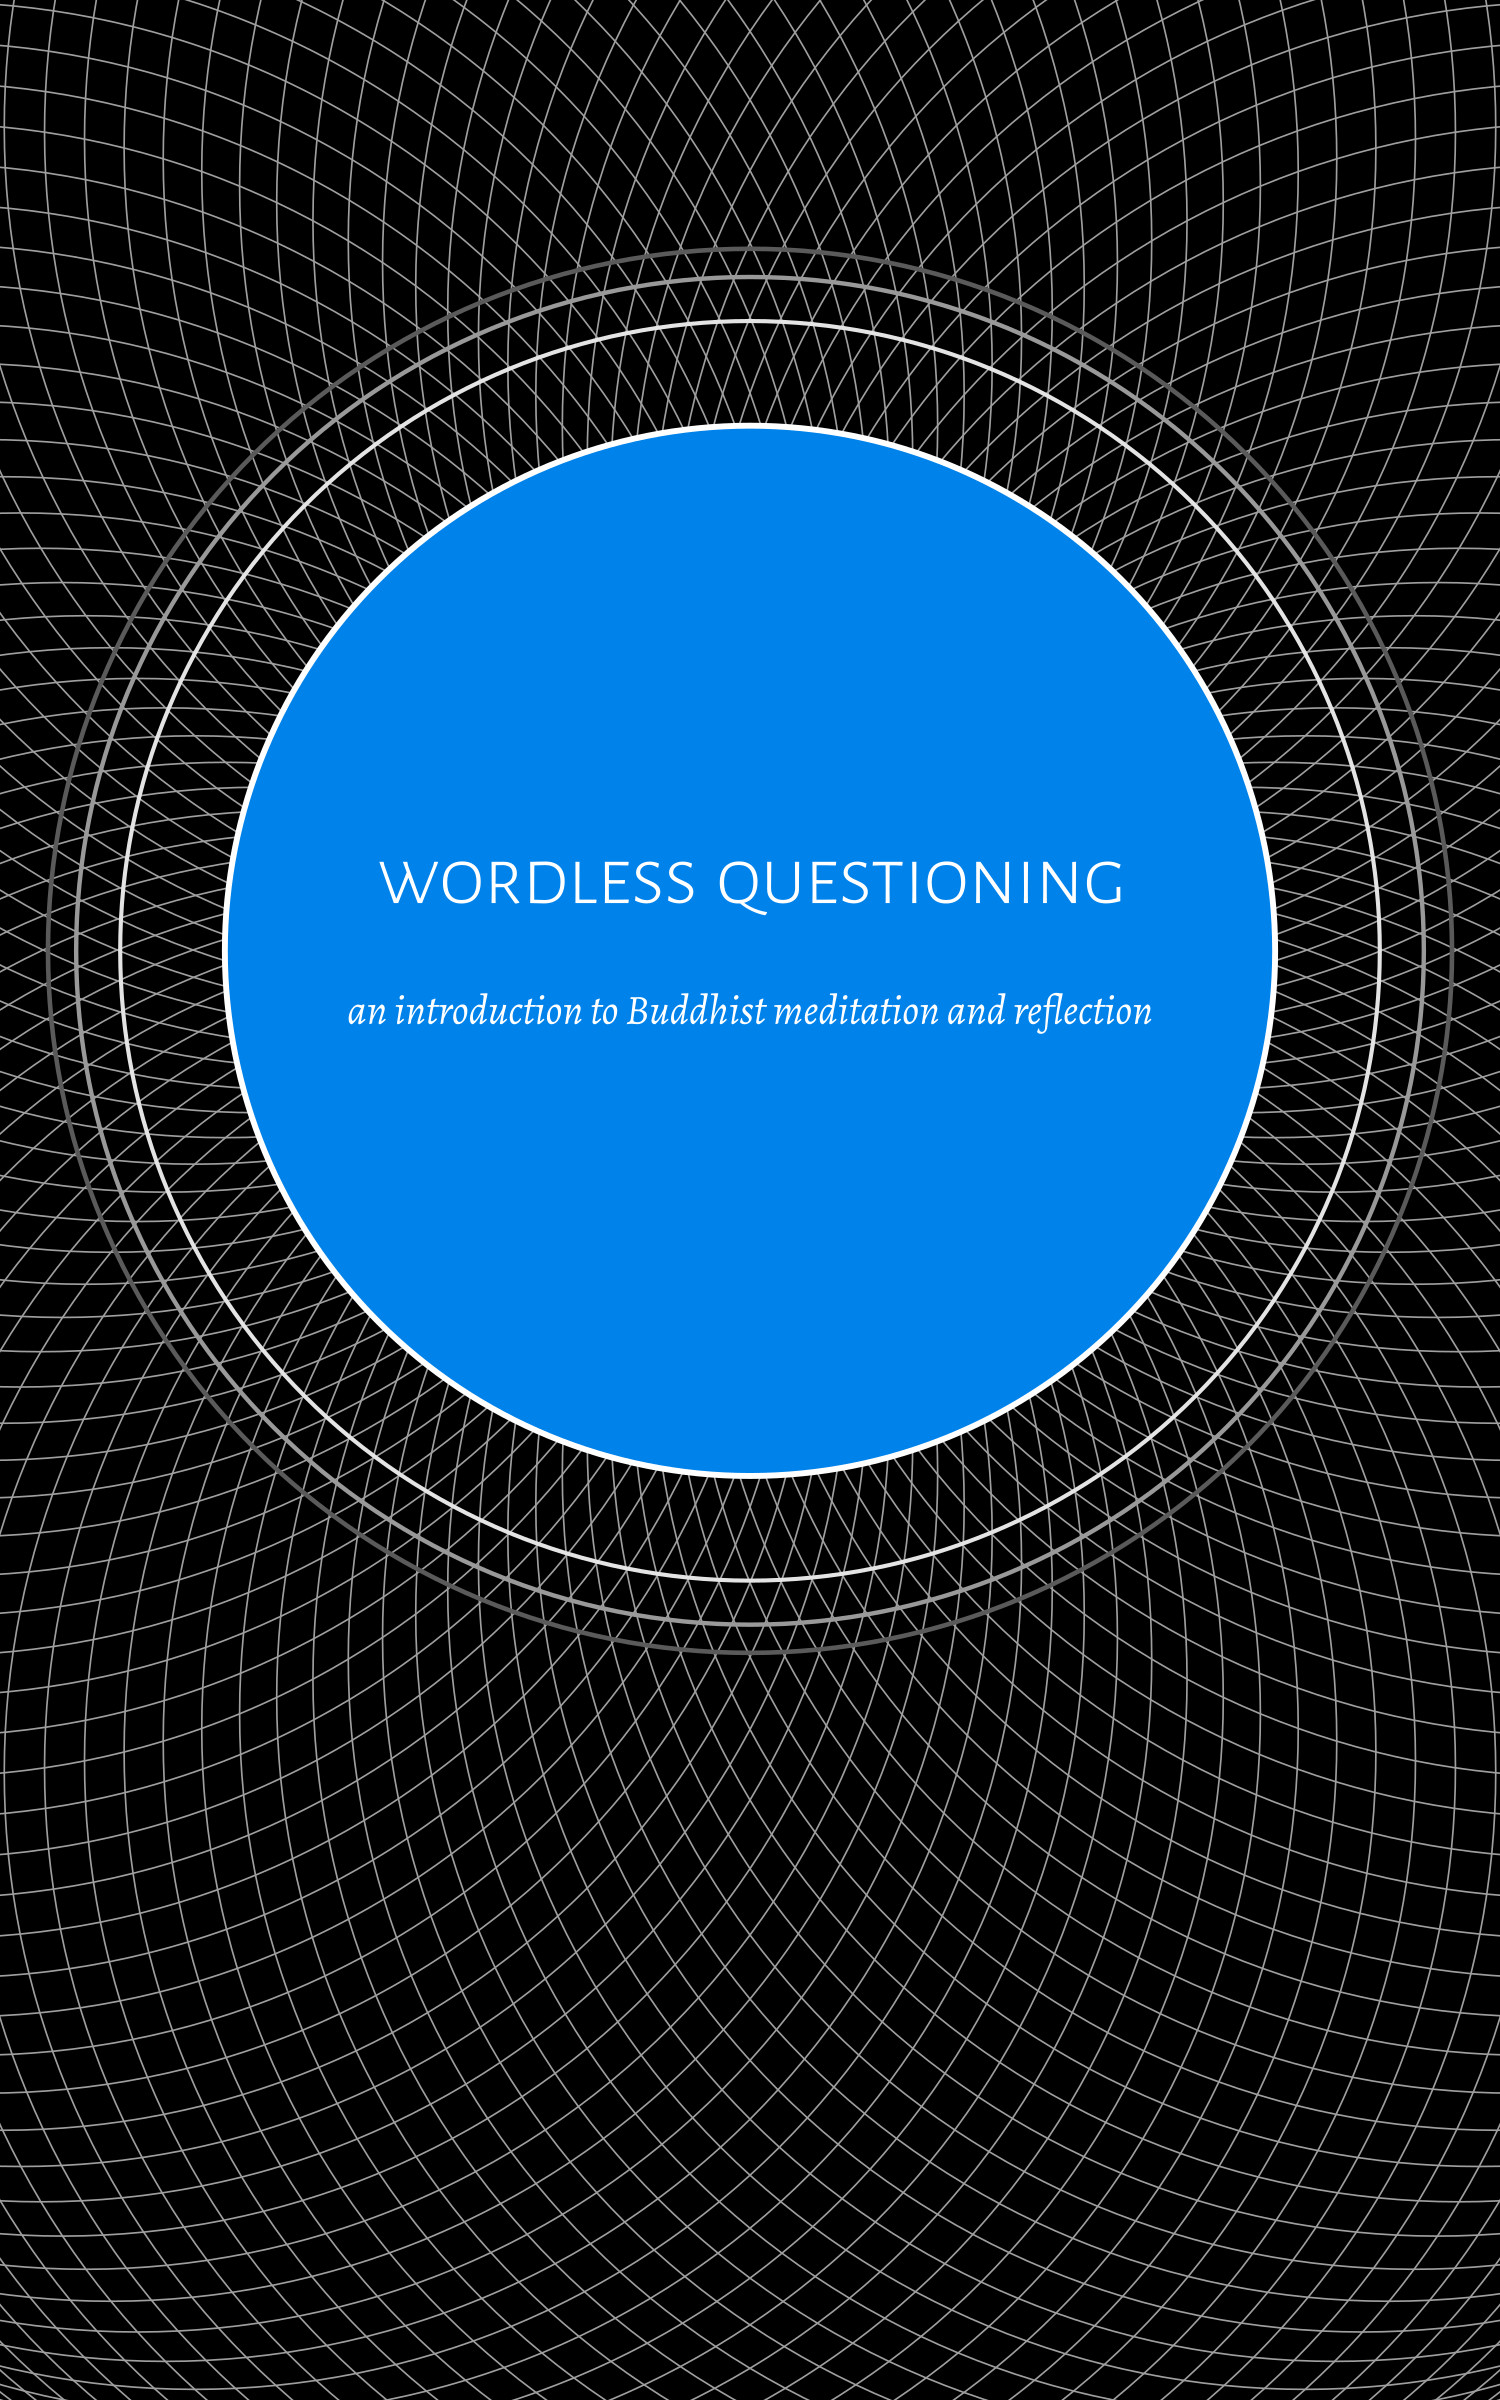
\includegraphics[height=\paperheight]{./desktop-cover-en.jpg}}
\fi

\cleartorecto
\thispagestyle{empty}
\vspace*{5em}

{\centering

{\Large\alegreyaSansScLightFont\selectfont\MakeLowercase{\textls*{\thetitle}}}\\[5pt]
{\chapterTitleFont\selectfont\itshape \thesubtitle}

\vfill

{\chapterTitleFont \theauthor}

\vspace*{2em}

}



%\cleartoverso
\thispagestyle{empty}

{\copyrightsize
\centering
\setlength{\parindent}{0pt}%
\setlength{\parskip}{0.8\baselineskip}%

\thetitle\\
by \theauthor

% Published by \thePublisher
% 
% ISBN \theISBN
% 
% Copyright \copyright\ \thePublisher\ 2019
% 
% Cover Photograph: The Person

\vfill

This work is licensed under a Creative Commons\\
Attribution-NonCommercial-NoDerivatives 4.0 International~License.

Produced with the \LaTeX\ typesetting system, set in Crimson Roman and Alegreya Sans.

% \theEditionInfo

}


%\cleartorecto
\thispagestyle{empty}

\mbox{}\vfill

\noindent
{\itshape
  \ldots\ The wise acts without haste,\\
  teaches without words,\\
  lets the waters flow, doesn't struggle\ldots
}

\bigskip

\noindent
{\smaller Tao Te Ching}

\vfill\mbox{}


\cleartorecto
\tableofcontents*

%\chapter{Introduction}

While I was studying at Budapest in 2005, I remember looking for books
which could help me get a useful perspective on my confused experiences.
There was no lack of explanation and advice, but they were missing a
concrete direction: `Interesting ideas, but what do I \emph{do} and
how?' I believe that good instruction should enable one to do more than
before, shed light on the `what' and `how', and even on the `why'.

The first book which gave me a tangible foothold was Ajahn Sumedho's
short book, \emph{The Four Noble Truths}.\footnote{\href{https://forestsangha.org/teachings/books/the-four-noble-truths?language=English}{The
  Four Noble Truths (forestsangha.org)}} It provided an introduction to
a practical method of investigation with examples of Ajahn Sumedho's own
struggles. Later, when I was staying at Amaravati Buddhist Monastery in
England, I read his other book \emph{Mindfulness: the Path to the
Deathless}\footnote{\href{https://forestsangha.org/teachings/books/mindfulness-the-path-to-the-deathless?language=English}{Mindfulness:
  The Path to the Deathless (forestsangha.org)}} and found it
illuminating as well.

I mention these books here because certain topics are covered in more
detail there, and if you are reading this book, they might also be
helpful.

Here, I collect advice and teachings that I wish I had read, or someone
had told me sooner, during the years since those early books. The right
answer remains obscured until we learn how to ask the right question.

I included diagrams and illustrations, which communicate on a different
channel than words, alongside the prose text. When I start drawing a
diagram, I discover relationships between terms which I hadn't thought
of before. When I see somebody else's diagrams, they show me how terms
are connected on a larger scale, and I ask where that representation can
be found on the map of my experience.

Illustrations of the meditation postures were carefully drawn by
Madalena Scafuro.

The Venerable Bhikkhu Kovilo carried out a large amount of editing work
on the text and converted my Hungarian-flavoured English into native
idioms and fluid phrases. I am grateful that they have dedicated their
time and energy to the project and this guide is all the better for it.
In regards to any part of this book which seem disorienting, unclear or
confusing, the responsibility and fault remain with me. Leave those
parts behind and return to learning from the Buddha, our incomparable
teacher. He taught the timeless truth, the complete ending of suffering,
because he had faith in our ability to recognize~it.

Over the years, I have received much help and support from my first
teachers, who are my parents, and from monastic teachers and friends. We
may feel inadequate and not believe that we can ever feel happy, but our
teachers believe in us and wish us to succeed, to overcome confusion and
flourish in our life. I offer these words in this spirit.

\bigskip

\enlargethispage*{3\baselineskip}

{\raggedleft
Gambhīro Bhikkhu\\
2021 November,\\
Sumedhārāma Buddhist Monastery, Portugal
\par}


% Page 1 is the first page of the first chapter.
\mainmatter

\hypertarget{breathing-1}{%
\chapter{Breathing}\label{breathing-1}}

We watch the sensations of the breathing in the body, this alert
attention collects and calms the mind. We watch, what do we feel in the
body when we breathe in, what do we feel when we breathe out.

Breathing in, we feel the cold air first at the tip of the nose, it
fills the lungs while the chest expands and the abdomen draws in
slightly. There is no need to control this. The body knows how to
breathe, for us it is enough to observe, like watchings waves wash in
onto the shore, and then recede.

We don't have to tell ourselves what to think and how to feel. If we
want clear thoughts, it is best to first be silent and listen. We sit
quietly for a little while, and when we are silent, the clear thoughts
will come their own, or the mind will be satisfied with the silence.

A clear, conscios thought is followed by peaceful gladness, the mind is
content and happy, doesn't feel the need for a lot of internal
discussion, it is satisfied to listen to the silence.

The right attitude is a careful balance. We establish a clear intention
to stay with the meditation and leave other matters until a later time,
but too much force becomes rigid and obstructive.

A clear mind and good aspiration feels settled and cool, open for
changes. A struggle of will-power feels busy and hot, narrow in scope.

I remember, I used to think that during meditation we are observing the
breathing because we are supposed to learn new things from it. I sat
down and struggled to understand how to do it, and kept thinking and
changing how to breathe, expecting that eventually it will somehow work,
and some day, doing it in the right way I will start learning new facts
about the mind. It was rather painful and mostly fruitless.

The best is when we have to learn something we didn't volunteer to
learn. We don't learn new facts from meditation, because there are so
few that we need, that we probably already know them.

But we don't stop to stay with them, and unpack their significance for
\emph{what to do}, \emph{in what manner to do it}, or in other words
\emph{how to be}. A list of facts, if not integrated, doesn't reach deep
enough to deal with root causes in the heart and mind, and have no
effect on us. Watching the breath stops us and opens the attention which
can do that.

The Buddha only has a simple message for us: wake up, stop holding on,
you don't have to suffer. We keep unpacking this, opening it wider and
wider.

Take a few minutes to adjust how you sit and find a balanced posture.
The important point is to be upright, in a stable but not tense posture,
with the head balanced and not lulling forward, and that your posture
should allow open, easy breathing.

Determine that you are putting down everyday activities for this period.
If such a thought interrupts you, respond, 'This is not the right time,
I will come back to that when the time is appropriate. At this time, I
am watching the body the breathing.' It's a bit longer than 'Go away!',
but more friendly to ourselves. It helps to think the thought
deliberately. This establishes a clear intention in the mind, like
clearing a desk before starting work. We are putting them down not
because they are not important, but because we care about doing our
tasks well. If we don't rest, we can't do our work well.

Take a deep breath and watch if you feel tension, something obstructing
or limiting the breath. If it moves easy and open, then your posture is
suitable. You don't have to sit in a special way.

Pay attention to the physical sensation of breathing. Let the body
regulate the breath, we only watch and let it relax, giving attention to
what is happening now.

Good posture and the calm, easy breathing is a quiet and pleasant
feeling, like sitting down on a park bench after a walk. There nothing
special to do, and this simple, quiet sitting is a joy in itself.

Breathing in, we first feel the air at the nostril. The cold air moves
down in the windpipe, fill the lungs, and the chest expands. The abdomen
muscles and diaphragm move inward and outward, controlling the movement
of the air. The quiet rhythm of heartbeats can be felt. Breathing out,
the muscles relax, the chest contracts and the rib bones move closer.
The warm air rises through the wind pipe, and exits the body through the
nose.

It is not necessary to express this in thought, relax and watch as the
feelings appear in the body. It takes a few minutes for the body to
settle. The beating of the heart will calm down, and the breathing will
become regular and light.

Allow the body to regulate the breathing on its own. When we approach it
with an opinion, that our breathing should be short or long, then it
becomes rigid and forceful. We want to discover our experiences, not
tell them what they should be.

The body knows how to breathe better than we do. It can do breathing for
us very well, if we let it. Rather than trying to figure out whether you
are breathing correctly or not, take a step back and turn the attention
around, listening instead of directing. Breathing in, breathing out,
what are you feeling in the body?

There is no specific thing which you have to experience. The intention
is rather to have the time and allow the space to be with your
experience.

Centred within itself, knowing the simplicity of the present moment. If
you feel that you have to complete, or fix something, it is always an
extra, something which we create. We create this expectation that we
have to change, we have to fix, we have to control. Notice that
compulsion and recognize that you can let it go, you don't have to do
that.

If there is a lot of tangled thinking, determine what to think, instead
of letting the mind run in circles. For example, use the mantra BUD-DHO,
which means 'the one who knows'. On the in-breath, think BUD-, on the
out-breath, -DHO. If we have already built up a strong momentum in the
thinking, and it refuses to quiet down, this puts down a guard rail and
speed bumps on the road, so that we stay on track and slow down.

Breathing in, staying with the simple experience of the moment, and this
is enough.

We feel compulsions, desires and anxieties, we feel 'I need this', 'I am
like this', 'I should be like that' -- they are something we can
observe. Staying with the breathing, we can turn attention to the
experience that is happening.

Awareness of the body is a solid base, calming and reorganizing what is
valuable. If your experience is peaceful, happy and content, stay with
that. There is nothing wrong in that. It is a happiness which is not
connected to craving, not dependent on having to get or reach something.
It is a happiness arising from seclusion of the senses, returning to
simplicity, knowing and staying with the present. The mind is alert,
content, and satisfied.

Meditation can bring up turbulent emotions, and that is good. We are
seeing what we haven't allowed ourselves to see. It is not necessary, to
look for answers or solutions, we investigate the emotions not on the
level of personal stories, but more fundamentally, as states of the mind
and heart. On that level there are no stories, the feeling or mind state
doesn't announce who it is and what it thinks of us, we are ones who add
that to it.

Generosity relaxes the mind, and morality establishes stability. We may
think of good actions, what we have given and received, we may recollect
people we look up to as good examples with respect.

If you find yourself in a tense, strict and cynical mood, I recommend
shift your posture slightly to relax, quietly rub your ears or massage
the face muscles using your fingers, and recollect generosity. In the
monastery, it is frequently the lay friends who come to cook and offer
the midday meal for the community. They can be busy while in the
kitchen, but when finished, they are at ease, relaxed and smiling.

Recollecting our good actions, even simple and small things, relaxes the
mind which is thirsty for results. Imagine what would happen, if someone
gave you a hundred-times-fold of what you need. How are you going to
meditate then? Probably much like now, just more relaxed. Grant yourself
that rich, wide space.

Generosity lets us recognize that we have space, and don't have to push
get ahead of others, there is goodness in the world and we can drop the
big hurry. It also feels joyful to recollect the generosity of our
family, relatives and friends, but even seeing a stranger help another
stranger brings us to smile.

'How can I do it?' Approach it differently, and ask instead, 'Can I pay
attention to it?'

You are only going to know it after the initial trust has allowed you to
practice, and you are only going to be able to express with knowledge
what is already behind you. That which is ahead, you can't describe it
precisely, thinking is not sufficient for that.

The sensation of breathing stops us. We are back at the beginning, when
we don't know what is going to happen. We are at an empty and spacious
place this way, where we are by ourselves and we have time to stop
there.

The senses turn inward when watching the breathing. The eye sees
colours, but the seeing is directed inward, it is not seeking col or and
forms outside. The ear hears sounds, but the hearing turns inward and is
not seeking. The body feels hot and cold, the surface of clothes and the
rigid weight of the bones. We watch this while breathing and let the
body calm down, let the mind turn inward and grow still.

Consider a lake which doesn't have inlets or outlets, contained all
around by the valley, its only water-source being a fresh, cool spring
in the ground. When it rains, some water will flow into the lake through
small channels, but there being no outflow, it will all settle in the
lake contained by the valley. The water in the lake remains still, and
the cool water from the spring will spread and permeate the entire lake.

Feelings and the mind are dependent on the body, we can't add to it or
take away from it. It is complete in every breath, it start with the
body and is going to end with it. This world, made of feelings, is
complete in this -- everything we are and everything we can ever become,
is contained in this.

When we suffer, we know that there is something we don't understand. We
don't understand how one thing was created by another, how one thing is
under our control, and another is not.

When we don't see, we repeat the same pattern like following a program,
and create the same suffering again and again. We complain, 'why does is
always happen this way?' We keep doing the same thing, and not see it.

Looking closer, we see that one thing depends on another. Then we can
see the option, that we are free to stop doing it. We return to a quiet
contentment that way.

When we have been sitting in meditation for a while, we often start to
complicate it. Where does this come from, that we can't stay with
something simple? Notice how belief in the simple changes, we start
thinking about some point, and the doubt and self-criticizing stops
everything.

It is comical, how we can be so committed to our self-criticism, as if
it was a transcendental experience to cause ourselves pain. But we feel
we should be struggling with \emph{something}, we should crush our ego
and let go of everything. Perhaps this is the only way we know, we don't
even know what it could be like to not be like this.

At the beginning we have the kind and flexible attitude to ourselves,
but there is only hardness and judgement at the end. The young tree is
pliant and fresh, it bends easily as it grows, but the old tree is hard
and dry when it dies.

Return to the beginning, where there is kindness to the beginner, where
you didn't yet expect yourself to know. We don't know what is here until
we look and see. That seeing and watching is the fresh knowing. Allow
yourself to be always at the beginning.

\clearpage

\begin{figure}[h]
\caption{Mindfulness of Breathing (\emph{Ānāpānasati})}\label{fig-mindfulness-of-breathing}
\bigskip\centering
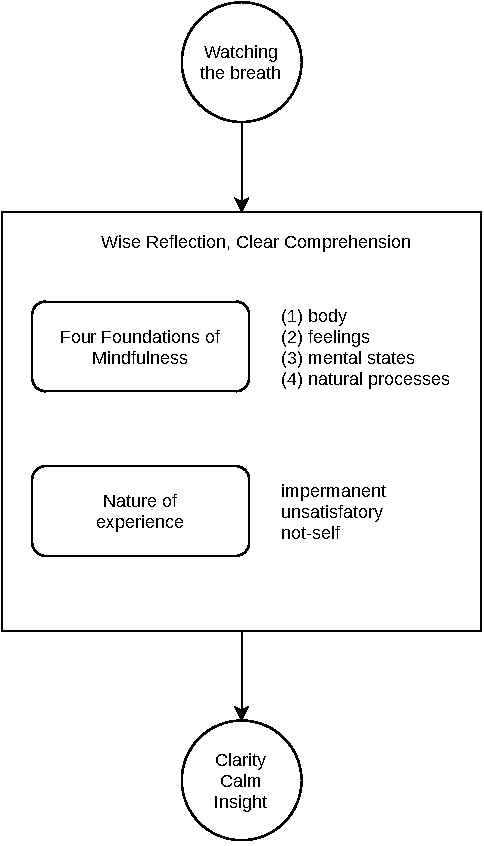
\includegraphics[scale=0.8]{mindfulness-of-breathing.pdf}
\par
\end{figure}

\clearpage

\section{Mindfulness of Breathing (excerpt)}

{\centering
\emph{\href{https://suttacentral.net/mn118}{MN 118}, Ānāpānasati Sutta}
\par}

{
\setlength{\parindent}{0pt}\setlength{\parskip}{5pt}
\fontsize{9.5}{14}\selectfont

Bhikkhus, when mindfulness of breathing is developed and cultivated, it is of great fruit and great benefit.
When mindfulness of breathing is developed and cultivated, it fulfills the Four Foundations of Mindfulness.
When the Four Foundations of Mindfulness are developed and cultivated, they fulfill the Seven Factors of Awakening.
When the Seven Factors of Awakening are developed and cultivated, they fulfill true knowledge and deliverance.

And how, bhikkhus, is mindfulness of breathing developed and cultivated, so that it is of great fruit and great benefit?

Here, bhikkhus, a bhikkhu, gone to the forest, to the foot of a tree or to an
empty hut, sits down having crossed his legs, sets his body erect, having
established mindfulness in front of him.

Ever mindful he breathes in; mindful he breathes out.

\textbf{Body}

Breathing in \& out long, he knows:\\ `I breathe in \& out long';

Breathing in \& out short, he knows:\\ `I breathe in \& out short';

He trains thus:\\ `I shall breathe in \& out experiencing the whole body'.

He trains thus:\\ `I shall breathe in \& out tranquillizing the bodily formations'.

\clearpage

\textbf{Feelings}

He trains thus:

`I shall breathe in \& out experiencing rapture'.

`I shall breathe in \& out experiencing pleasure'.

`I shall breathe in \& out experiencing the mental formations'.

`I shall breathe in \& out tranquillizing the mental formations'.

\textbf{Mental States}

He trains thus:

`I shall breathe in \& out experiencing the mind'.

`I shall breathe in \& out gladdening the mind'.

`I shall breathe in \& out concentrating the mind'

`I shall breathe in \& out liberating the mind'.

\textbf{Nature of Experience}

He trains thus:

`I shall breathe in \& out contemplating impermanence'.

`I shall breathe in \& out contemplating the fading away of passions'.

`I shall breathe in \& out contemplating cessation'.

`I shall breathe in \& out contemplating relinquishment'.

\bigskip

Bhikkhus, that is how mindfulness of breathing is developed and cultivated, so that it is of great fruit and great benefit.

}

\chapter{Understanding}

\keywords{facts and experience, doubt, accumulating facts}

\noindent Though we break knowledge into parts and we speak about
practice in gradual steps, understanding happens all at once. Perception
is immediate -- the `Aha!' moment, when the fog clears. While some
information is necessary to begin, we remember that the truth of the
teaching is `to be experienced for oneself'. In meditation practice, the
facts which are useful for us are \emph{here-and-now} facts which we can
know in our present experience.

If we depend solely on external information or simply wait for some
experience to arise, we never arrive at the place where we can stop.
This dependence is exhausting. It keeps creating more doubt and mental
restlessness. Even though we accumulate more facts, we can become
bitter, and this inner feeling of lack grows. It is not more information
that we need, but the letting go of that need. Then, we are able to stop
in peace.

\keywords{sense experience, identification}

Memories, perceptions and expectations create a force which pushes and
pulls on us. While the experiences themselves disappear, the compulsion
never rests: we already want the next one. How can these phenomena be so
convincing that they keep pulling us forward? What keeps feeding the
process is that \emph{we see ourselves in them.} We see them as what we
are, what we were, what we are going to be. And since they keep changing
and breaking up, we continue on and on, expecting the next one.

\clearpage
\figurepagelayout

\begin{figure}[h]
\caption{Feeling and Identification}\label{fig-feeling-identification}
\bigskip
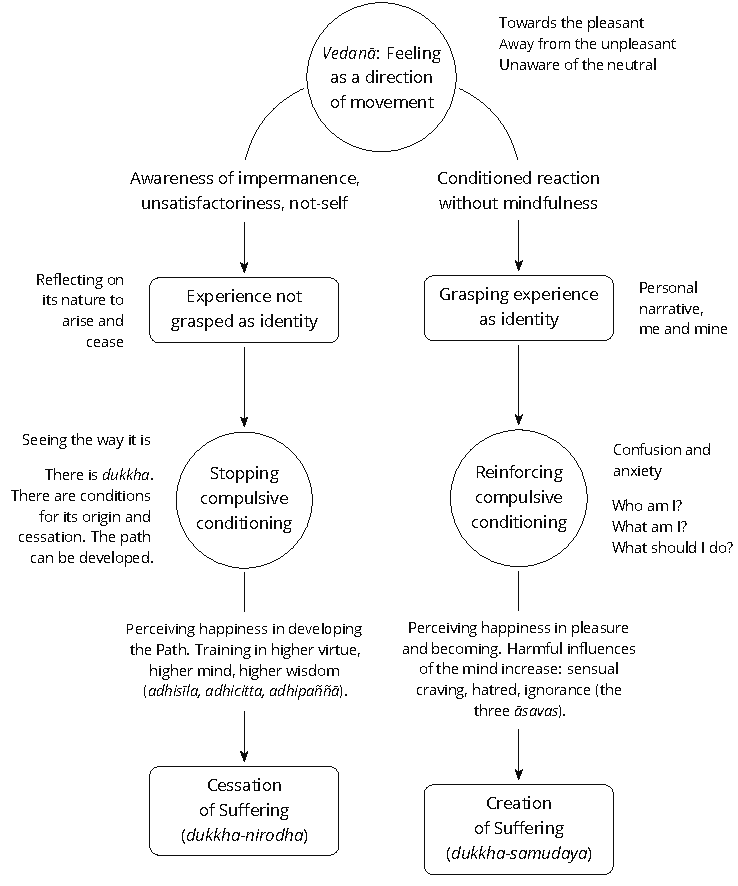
\includegraphics[width=\linewidth]{./manuscript/tex/diagrams/feeling-identification.pdf}
\end{figure}

\clearpage
\normalpagelayout

What if we woke up one morning without any memory of our past? Even in
that state, we would still grasp our experience as \emph{me and mine}.
It might be so disturbing that we would just lie there paralysed with
fear until we were able to grasp some story that could explain where and
who we were. In reality, we don't have to lose our memory to witness
this: missing an important flight connection or any other time when we
can't control our situation can be frightening enough to cause us to
feel this way.

It is humbling when we notice how much we take personally, even though
intellectually we know we shouldn't. The Buddha teaches that the mind
continues to construct `me and mine' out of sense-experience until the
impermanence of this experience is fully comprehended. We are taking it
personally if we are convinced that either (1) `This is me', (2) `I am
in this', (3) `I am outside of this', (4) `This is mine', or (5) `I
delight in this'.\footnote{\href{https://suttacentral.net/mn1/en/bodhi}{MN
  1}, The Root of All Things}

Oh, poor mind, why can't we be wiser? To start with, there is little
extra attentional space left when we habitually occupy our minds with
thinking about how to get what we want and complaining about what we
didn't get.

When the sense-base meets a sense-object, if attention is present, we
feel the experience as one of three feelings (\emph{vedanā}), comparable
to a direction of movement: toward the pleasant, away from the
unpleasant, at peace with the neutral. The untrained mind mechanically
follows these established patterns and gets caught up in the underlying
tendencies of passion, hatred and unawareness.

In this context, one understands feelings when one understands
sense-contact. As a result one sees the pleasant as painful (due to its
ultimately unsatisfactory nature), sees the painful as a dart (to be
removed or endured skilfully), and sees the neutral as impermanent (not
being lulled to unawareness).

This implies we don't conceive them as `me and mine'. We know them, but
the knowledge is not \emph{ours}. They don't belong to a person who
\emph{has} the feeling.

\begin{quote}
Having fully understood feelings,\\
He is taintless in this very life.\\
Standing in Dhamma, with the body's breakup\\
The knowledge-master cannot be reckoned.

\bigskip

\quoteRef{%

\href{https://suttacentral.net/sn36.5/en/bodhi}{SN 36.5}, Should Be Seen

}
\end{quote}

\keywords{thinking, being burdened, sense-restraint}

We can think a lot about this, but if we are trying to understand it
analytically, we will only give ourselves a headache. This understanding
has to be developed through the body: a good place to start is through
practising sense-restraint.

We guard the sense-doors. Clear comprehension will keep a space, a gap
between our awareness and its contents. When seeing a form, hearing a
sound, etc. we don't grasp at the experience, neither what we see as a
whole, nor at a particular feature we like or dislike. We might like the
experience, but we don't become enchanted by it. We might dislike it,
but we don't work up anger over it. We can keep part of our awareness on
the sensation of breathing, or maintain a broad awareness of the body --
this helps to find an anchor, a stable point, which informs our wisdom
faculty. If not the breath, it also works well to notice an aspect of
your current activity, such the touch of the pen as you write, the
pressure of feet on the ground or other sensations of the body.

This body-based practice is more simple than an intellectual approach.
It collects our mental energies and, with natural rhythm, results in
either calm stillness or thoughtful reflection.

We can notice that we are able to stop and that what we have with us now
is enough. Consider: in terms of objects and information, what have you
actually used today? Although you may own much, for one day, a little is
enough. We don't need as much as we think and relinquishing is not so
much a loss, as a relief from a burden. In this restraint we find
strength and energy which had previously been consumed by distracted
desire. Restraint is always at hand. It is not threatened by external
factors.

This is like learning how to pack less in your backpack for a hike.
After some experience, you can't even comprehend why you needed to carry
so much. Virtue is action that leads to happiness, and it can be
directed towards ourselves: relinquishment is one such personal virtue.
Understanding informs this virtue, and the happiness born from it
further supports trust in that understanding.

\clearpage

\vspace*{-\baselineskip}

\keywords{ānāpānasati, sense contact, sensation, feeling}

We watch the breathing, and observe how the senses operate. The eye sees
forms, and a sensation appears. The ears hear sounds; the body feels
solidity, hot and cold. If there is contact between a sense-door and a
sense-object, sensation is going to arise. The process doesn't depend on
us, if there is contact, we can't choose for the sensation not to arise.
When the contact between a sense-door and a sense-object is broken,
sensation ceases. The arising and ceasing of phenomena dependent on
contact -- this was our experience. Although we may have a measure of
control over our movements, other than that, we don't have a say in the
process of experience: it is not about us.

When we don't notice this, we think that the sensation is ours. If the
sensation feels good, we expect we are going to get something from it
and so we cling to it. This incorrect understanding of things underlies
our neediness and anxiety. When our expectations are disappointed, our
tendency is to assume that we did something wrong or that somebody else
made a mistake. We then go and search for some other experience which
will be more right, hoping that this new one doesn't play out like
before.

Observing sense-contact this way, feelings are no longer attractive or
repulsive. Instead, we see that neither inclination is stable or
reliable. This is not numbness. In meditation we turn toward experience,
not away from it. We cultivate attention with sensitive equanimity.
Though we remain alert and responsive to the experience, it no longer
controls and disturbs us. We remain calm.

\clearpage
\figurepagelayout

\begin{figure}[h]
\caption{Sense Contact and Feeling}\label{fig-sense-contact-feeling}
\bigskip
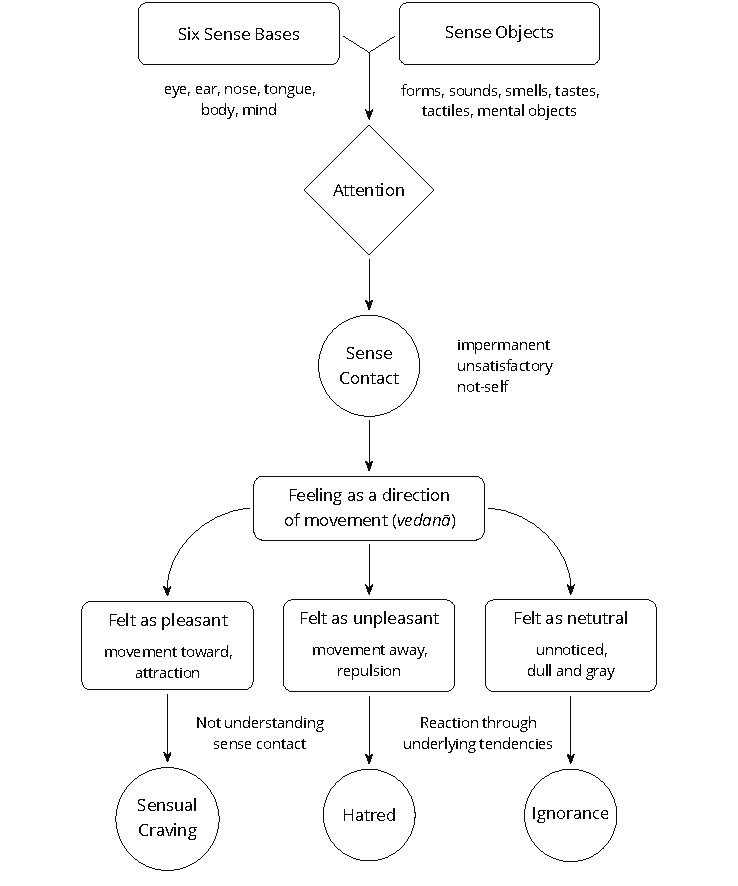
\includegraphics[width=\linewidth]{./manuscript/tex/diagrams/sense-contact-feeling.pdf}
\end{figure}

\clearpage
\normalpagelayout

\vspace*{-\baselineskip}

\keywords{self-narrative, self-description}

How does this affect the way we narrate experiences to ourselves? We
explain to ourselves that some feeling was good or bad and we describe
how we should think about it. The central element of this narration is
\emph{our feelings}, and its primary thrust is how to get more of the
good ones.

What happens when we realize that both the good and bad feelings we
experience are unstable and unreliable, and that their arising and
ceasing are not in within our control? Our internal values are
re-ordered, guided by impermanence, rather than craving.

\keywords{changing nature, wise reflection}

Usually we only start to pay attention once we have noticed that
something is wrong, or that something hurts, or that we are suffering.
We don't feel a great need to explain pleasant experiences, do we? We
can use the sense of frustration, the unsatisfactoriness and the
proliferative thinking as a sign to start mindfully investigating.

Mentally take a step back and observe that the experience is a process
which arises, persists in change, and ceases. Ask yourself: `Where in
the body do I feel this sensation? Can I remember when it started? Can I
see how it changes? Can I catch it as the feeling ceases?'

Although we can't control the world around us, our attitude influences
what we see as being free choices. Our perspective opens or closes the
doors toward the actions we see as possible. These actions create the
situations in which we live and influence how we see ourselves therein.
Without reflecting on the nature of our experience, we will be inclined
to see pleasant feelings as a reward and unpleasant feelings as
punishment, and the meaning of our lives will revolve around these. Our
inner world will constantly revolve around the questions of: `Who am I
\ldots{} How do I \ldots{} Why do I \ldots{} What should I \ldots{}' And
doesn't that feel like a burden better left behind?

Wise- and unwise reflection are terms in the \emph{suttas},\footnote{\href{https://suttacentral.net/mn2/en/bodhi}{MN
  2}, All the Taints} making a distinction between a superficial
attention that increases our confusion, and thorough investigation that
leads to clarity and correct understanding. Unwise reflection misses the
signs of impermanence, unsatisfactoriness and not self, hence getting
caught up in taking everything personally. Wise reflection notices these
characteristics of sense-experience, and investigates in line with the
Four Noble Truths.

\keywords{attachment to self, dog tied to a post, reflection}

Do you remember, how a dog, tied to a post with a leash is running
round-and-round its post? It sits, stands, walks or runs around it, but
everything it does is around that post.\footnote{\href{https://suttacentral.net/sn22.100}{SN
  22.100}, A Leash} This ego-driven proliferation is the same. Although
it keeps us busy, we remain attached to the self at the centre, not
being able to go anywhere else. The leash is the identification and
clinging (\emph{upādāna}), the process of formulating `me and mine' in-,
or around sense-experience, which in truth has no such essential
attribute. This leads us to unwise reflection centred on who we are,
what becomes of us, increasing our doubt and confusion.

Questions rooted in `me and mine' are a trap. They drag us on and on
without ever leading to freedom or stopping. If we find ourselves tied
to a post, what are we to do? Cutting the leash seems a good idea.

In the context of meditation, reflection doesn't necessarily include all
kinds of thinking. Not all thoughts are productive for insight. In
reflective meditation, we break down our experience into
cause-and-effect processes using the Four Noble Truths\footnote{\href{https://suttacentral.net/sn56.11}{SN
  56.11}, Setting in Motion the Wheel of the Dhamma} as a guide.

This begins with an experience that is personally easy to identify:
suffering, stress, unsatisfactoriness, or \emph{dukkha} in the Pali
language. The direction of thought is not towards \emph{my suffering} as
a personal history, but instead, observing it as an impersonal, natural
process.

\keywords{dukkha}

The starting position is to recognize that stress or suffering \emph{is}
here. As information, this is trivial: yes, there is stress and
suffering in the world. But when we ourselves experience it, we rather
like to pay attention to something else, or we tend to blame somebody
else for it. We will do any number of things rather than becoming
conscious of it and deal with it.

The instruction here is that the way forward is to turn toward suffering
and to investigate it. We seek a way of understanding. This is the First
Noble Truth in the teaching of the Buddha: there is suffering, and the
noble attitude is to turn toward it and understand it.

What do we understand? That this suffering is the result of earlier
causes and didn't arise from nothing. Examining our situation this way,
we are not helpless. Though we may not understand every little aspect of
our condition, it is already a relief to realize that we are, perhaps,
able to change something.

\clearpage

\vspace*{-\baselineskip}

\keywords{origin of dukkha}

The Second Noble Truth points out that the cause of suffering is in
ourselves. It is our wish that experience were otherwise than its nature
dictates. It is our tight clinging to what is impermanent, fragile and
not possible to keep. The suffering, the \emph{dukkha} that we
experience depends on that clinging and thirsty craving. The
instruction, the noble attitude here is to let go of this thirsty
craving and clinging because clinging to transitory experiences is
suffering.

\keywords{cessation of dukkha}

With the cessation of the cause, the result -- the suffering -- ceases
as well. The good news is that the end of suffering is also found within
ourselves.

From this perspective, we can see that the mind creates the kind of
world we live in. If we watch it, we at least have a chance to not make
the situation worse. And who knows, we might make it better?

The Third Noble Truth directs our attention toward this: there is a
solution; we are not obliged to live in bitterness and meaningless
struggle. The advice, the noble attitude is to practise and experience
this for ourselves through understanding and letting go of attachment.
In this way, we allow the suffering to cease.

Even if we can't fully let go right away, it is already a relief to see
that this connection is true: `If I could let go, I wouldn't suffer from
it'. This is already half the work. Until this point, we have been
wandering without a map. But now there is a way forward.

\keywords{path of practice}

\enlargethispage*{\baselineskip}

The Fourth Noble Truth describes the practice of the path. The Buddha
divided it into eight factors, which incorporate the situations of
everyday life and the development of meditation.

\clearpage

The parts of the Eightfold Path are (1) understanding, (2) intention,
(3) speech, (4) action, (5) livelihood, (6) effort, (7) mindfulness and
(8) concentration. When a factor is aligned with the truth, we call it
\emph{right}: Right Understanding, Right Intention and so on. Breaking
the path down into parts helps investigation and makes it is easier to
understand, but the path factors are not separate: they strengthen and
support one another. The practice is realized as an integrated whole.

When we most need the practice, we need it \emph{fast.} We can't stop to
count factors. The most useful tools are those which are portable and
most easily accessible in a given situation. When we read and ponder the
meaning, we have time to turn the words this way and that. This is the
stage of study. But mindful attention as an abstract idea doesn't help
much, it is most valuable when practised, when it is at hand in the
present moment.

We always return here. We remember the past and plan for the future, but
remembering is a present experience, and planning is a present
experience. We don't practice meditation for a future state. If we see
understanding, freedom, happiness and overcoming obstacles as some
future state, we only have more burdens. Letting go takes place in the
present, where states are changing without us.

\clearpage

\section{All the Taints (excerpt)}

{\centering
\emph{\href{https://suttacentral.net/mn2/en/bodhi}{MN 2}, Sabbāsava Sutta}
\par}

{
\setlength{\parindent}{0pt}\setlength{\parskip}{5pt}
\fontsize{9.5}{14}\selectfont

\emph{(Abandoning the taints is for one who knows wise attention)}

Bhikkhus, I say that the destruction of the taints is for one who knows and
sees, not for one who does not know and see. Who knows and sees what? Wise
attention and unwise attention. When one attends unwisely, unarisen taints arise
and arisen taints increase. When one attends wisely, unarisen taints do not
arise and arisen taints are abandoned.

\emph{(The uninstructed person falls into the thicket of views)}

This is how he attends unwisely:

`Was I in the past? Was I not in the past?'

`What was I in the past? How was I in the past? Having been what, what did I become in the past?'

`Shall I be in the future? Shall I not be in the future?'

`What shall I be in the future? How shall I be in the future? Having been what, what shall I become in the future?'

Or else he is inwardly perplexed about the present thus:

`Am I? Am I not? What am I? How am I? Where has this being come from? Where will it go?'

When he attends unwisely in this way, one of six views arises in him.

The view `self exists for me'\\
arises in him as true and established;\\
`no self exists for me'\\
`I perceive self with self'\\
`I perceive not-self with self'\\
`I perceive self with not-self'\\
`It is this self of mine that speaks and feels and experiences here
and there the result of good and bad actions; but this self of mine is
permanent, everlasting, eternal, not subject to change, and it will
endure as long as eternity.'

This speculative view, bhikkhus, is called the thicket of views, the
wilderness of views, the contortion of views, the vacillation of views,
the fetter of views. Fettered by the fetter of views, the untaught
ordinary person is not freed from birth, ageing, and death, from sorrow,
lamentation, pain, grief, and despair; he is not freed from suffering, I
say.

\emph{(The noble disciple reflects wisely)}

He attends wisely:\\
`This is suffering';\\
`This is the origin of suffering';\\
`This is the cessation of suffering';\\
`This is the way leading to the cessation of suffering.'

When he attends wisely in this way, three fetters are abandoned in him:
personality view, doubt, and adherence to rules and observances. These
are called the taints that should be abandoned by seeing.

\enlargethispage*{\baselineskip}

\emph{(Conclusion)}

Bhikkhus, when for a bhikkhu the taints that should be abandoned by seeing
\ldots{} restraining \ldots{} using \ldots{} enduring \ldots{} avoiding \ldots{}
removing \ldots{} developing \ldots{} then he is called a bhikkhu who dwells
restrained with the restraint of all the taints. He has severed craving, flung
off the fetters, and with the complete penetration of conceit he has made an end
of suffering.

}

\chapter{Cycles}

\keywords{steps in practice, descriptions and awareness}

Meditation teaches understanding through attention to feelings and
experiences in the present. The instructions often describe a
step-by-step development, but in the present, only one moment is
available to us. Are we taking a step forward or backward? Either way,
the experience is one step at a time, the step where everything is
changing. We use words to describe experience, but awareness of that
experience is wordless. Mindful attention is actively looking inward as
if asking a question. Even the symbols of language are limiting. While
they consist of fixed representations, the experience is in motion.

Perfecting the steps of the instruction is not the purpose of
meditation. The purpose is clear knowing of present experience, this
restores right perspective. We can develop the impression that we must
always complete the same sequence of steps, and when the mind doesn't
develop according to that sequence, we feel disappointed.

\keywords{narrating mind, experience as the basis}

And worse, other people seem to be meditating peacefully! They must have
got it right! The practice brings self-doubt to the surface. We may
consider it from the other direction: Someone might compliment us, `You
looked so peaceful, I'm sure you know something!' But, knowing how much
distracted thinking was going on in our head, we can see how unreliable
these impression are.

The narrating mind keeps mechanically making comments which are devoid
of any depth or investigation. The value of taking this step back is in
getting a taste for how unreliable and uncertain your own thinking mind
is, even when you think `I'm sure about this!'

Turn that attitude around and start with experience. Begin with a
questioning, curious attention that wordlessly inquires about the
present. If we take our experience as the basis, the way this experience
is now, what understanding does that give us? We look at ourselves first
-- how are we feeling? what state are we in? -- and respond
intelligently to that with cultivating our meditation in the right
direction. When painting a wall, we look at the wall first, choose the
right paint for it, and \emph{then} follow the advice on the paint can.
The wrong kind of paint will peel off, won't it? There are times when we
need to calm down, other times we need to generate energy and effort, or
wait for an internal storm to pass.

The various steps of any meditation technique are a method of learning
through imitation. Following an example, we watch ourselves and see how
our minds work. When we feel suffering, either we are able to resolve it
or we wait it out with patient endurance until it ends. Once it passes,
we look back with a clear head, knowing what had happened and by what
cause. In this way, our confidence in the practice will grow. We have
learned something there, and we don't need to hold on to the details of
the introductory example.

\keywords{development in cycles}

This would be a simple task, if our meditation practice developed along
a straight line, in direct proportion to the minutes and hours spent
practising. We plan that we are going to sit down, perhaps a bit
distracted at the beginning, but after an hour, \emph{if we are good
meditators}, we are going to feel stillness and our mind is going to be
clear and focused. At least this is what we expect.

Later, as we recollect how the meditation went, we observe that this is
not what happens. Our experience doesn't develop in a linear way from
shallow to deep or from distracted to focused. We might think that this
is our fault, because we are not `good meditators', or because we are
not doing the steps `right'.

As soon as we try to follow a technique step-by-step, everything starts
happening differently from our expectations. We might think, `Am I not
trying hard enough?' We keep pushing and it keeps getting more painful.
This is the feeling of trying to fit an opinion onto the experience.

If we look back at how our experience changes over time, we see a
different pattern. Experiences arise, change, cease, and are followed by
other experiences. The mind develops in cycles like this, and these
cycles ignore our goals of wanting to develop our meditation like a rank
ladder. The commenting mind tries to fit a personal story onto the
experience, about us being somebody who is good or bad at meditation.

Instead, we can take our experience as ground truth and start from
there. What kind of experience is this? We can notice how attention
moves as a process in consciousness and how it progresses through
different cycles.

Initially, the mind is content to sit, resting with relaxed attention,
just like when sitting down on a bench after a walk: sitting and
breathing is peace complete. But thoughts start coming up and we follow
them. We stop and remain content with the stillness again, thinking
might even stop without us noticing that we are not thinking. But
attention starts moving and we notice ourselves thinking again.
Memories, desires and restlessness can come up and we notice we have to
work on these. Then, the mind is again content and returns to the
feeling of stillness.

\keywords{knowledge and knowing, naming process}

Some knowledge is necessary, but a little is enough. Remembering the
teachings of the Buddha is a treasure which doesn't run out. But the
insights and understanding doesn't become \emph{our knowledge}, as
something we own from that point on. We can't put the truth in a box and
store it for next time, instead, we continue recognizing it in the
present. When we create fixed ideas from what we think we already know,
the practice looses touch with reality. Every time we start again from
the beginning, and from there, we trust the present knowing.

Facts and statements are attractive to the thinking mind, we feel a kind
of security in reciting facts. We would like to say, `I had a good
meditation', `I had a bad meditation.' We want to create distinctions
and to name our experience.

This is the dissatisfied mind. It wants to become something, it wants to
arrive at a state and have a name. But there is nowhere it likes to
stop. It goes on and on until we notice that, in this constant running,
we are completely exhausted.

When it becomes apparent that we are the ones doing this, the naming
stops. It stops because seeing replaced not-seeing; knowing replaced
ignorance. Consciously seeing the naming is enough to stop the
compulsion from continuing.

In the present, everything is changing, nothing is static. Everything
moves, experience is turning and flowing. It doesn't pose for a photo
and wait for us to name it. In this change, the doubtful and anxious
questions, identity and goals dissolve and lose their meaning. Using the
phrase in the \emph{Mahāsatipaṭṭhāna Sutta}, `He dwells independent, not
clinging to anything in the world.'
(\href{https://suttacentral.net/mn10}{MN 10})

This is enough, knowing the mind this way we stop and arrive at a place
where we can be grateful for being. Not a for anything in particular.
Being grateful that there is experience, knowing, clarity, and the
freedom which allows us to stop going towards more and more.

\keywords{ambiguity, limited symbols, knowing without naming}

In a balanced posture, the subtle feelings of the body are easy to
observe. With a curious attitude, we direct attention inward. We don't
know ahead of time what we are going to find.

These feelings are often not clear. We experience them but they don't
have clear boundaries. They don't have edges, or a definite shape. We
try to find words for them, but they don't fit. We are not sure what to
call them.

All symbols which could be used as a name are lacking. In our western
culture, we have strong trust in facts, and we like to return to that
security through terminology by giving things a name. We are not
familiar with the type of cognition that doesn't use names and fixed
symbols. Although the feelings and the experience as a whole are not
precisely defined, we know that this experience is present.

This way we can distinguish the naming process from the experience
itself. The subtle feelings in the body are nebulous, they don't have
clear boundaries. While breathing in and breathing out, we can
experience what the body as a whole feels like -- everywhere at once.
The whole body is breathing. There is feeling and experience, but there
are no names and clear boundaries.

We drop the naming process and recognize that we can know these feelings
as they are present. The knowing mind is glad to widen its scope and
include experience without filters. We can know what experience is like
without having to find a name for it.

\keywords{contemplating the mind, too much thinking}

Accompanying unwholesome mental states, we can notice sensations of
heat, restlessness, dissatisfaction and anxiety. We remember to turn
toward it with patience, and maintain endurance while this state goes
through its stages. This too will change, this too will end, and we can
wait for it. When we know where we are, in most cases this is enough.
Processes in the mind will change on their own. If we are not putting
fuel on the fire, it will burn up what it has and will go out on its
own.

Resolution and repetition are part of the practice, but in striving
towards a specific goal, the effort becomes bitter and tedious. `Is this
complete awakening yet? Or at least a bit? When is the meditation bell
going to ring?' Don't look for a state. The mind which tries to become
awakened is overcomplicating the situation.

Present experience is always simple, and mindful attention has a
capacity for wise understanding. In this practice, we keep returning to
it, this is what guides the effort.

We can't force this by will, and we can't guarantee what will happen: we
have to trust the process. What remains is a wholesome mind which
understands what is happening. We are not rushing with compulsion nor
forcing our way through things. After the difficulty, we have space for
gratitude to appear. We can appreciate the feeling of coolness and the
comfort of being at ease.

\keywords{integrated practice}

We look at our teachers as examples. They didn't meditate to achieve
some special state and then look for something else to do. Meditation
was not separate from, but was integrated into their lives. In examples
from the suttas, the traditional scriptures of Buddhism, the Venerable
Sāriputta's practice was to stay with the perception of
emptiness.\footnote{\href{https://suttacentral.net/mn151}{MN 151}, The
  Purification of Alms} The Buddha is portrayed as maintaining his mind
in concentration on the signless. This is how they continued to
meditate.

\chapter{Boat}

\keywords{walking meditation method}

\noindent Walking meditation is a more energetic alternative to the
sitting posture. Find a path, or an area with enough free space to take
a few steps, walking back-and-forth. Even though we are walking, our
attention is directed inward. We are not walking \emph{to} some place,
we are using the walking posture to develop the mind.

An outdoors, private location is ideal, but indoors in a large enough
room is also good.

Determine two points with a clear path between. This could be two trees,
or a couple of pieces of furniture. A short path might be fifteen paces,
a longer one about thirty paces long. Stand at one end, and start
stepping toward the other end mindfully with a clear intention to stay
with your meditation object, such as the breath, or the physical
sensations of the moving body. Keep your gaze lowered, looking at a few
steps in front of you. At the other end of the path, stop and wait for a
couple of breaths. Keeping your intention immersed in the meditation,
turn around, and start walking in the other direction.

Hold your hands in a way that allows you to maintain the continuous
inner attention. Most people prefer clasping the hands in front. It is
not the exact position that matters, but slinging the hands around tends
to be distracting.

\clearpage
\thispagestyle{empty}\mbox{}
\photoFullBleedPlaceholder{%
  TODO: Illustration of walking meditation.%
  \illustration{Walking Meditation Posture}%
  \label{illus-walking-meditation}%
}
\clearpage

Adjust your walking speed to suit your energy level and meditation
object. Some people do walking meditation with fast and determined
steps, other people take slow and careful steps. The suitable speed may
change even during one session. Experience the variations and find what
suits your practice and mental background at that time and place.

\keywords{manipulating feelings, self-importance}

Walking meditation used to stress me out. I believed that it was useful,
but that the technique was too loose and didn't involve precise enough
details about how to do it. I felt I wanted a checklist to go through
and verify if I was doing it right or not.

I kept wanting to walk \emph{to somewhere} so that I would \emph{feel
different}. I would start a walking meditation session between two
trees, but it felt like I was not doing anything, so I kept changing how
I walked to manipulate how I was feeling. `Walk faster, that will be it.
Slow down, and focus. Try breathing like this, and stepping like that,
until it feels different.'

It was also important that other people saw that I was doing something
important. So I would walk back-and-forth until I started to wear a
visible track in the grass on the ground. That was the proof, `I have
done something, I can see it, and \emph{they} can see it!'

Notice how much this kind of struggle is driven by the question, `How
can I feel better about myself?' The motivation is centred on
\emph{manipulating} feelings, not on \emph{understanding} them, how they
arise and cease. Self-importance is not a helpful attitude for practice.
Our desire identifies some external sign and it becomes terribly
important for us to see it, and to let others see it as well. That
\emph{important} track in the grass I made (which probably disappeared
by next dawn) is one example. Articulating it to ourselves when this is
happening already changes our attitude toward the process.

A helpful attitude to practice can be to approach it as if we were doing
something completely ordinary, but to bring along a sense of exploration
and to remember that the benefit is not a wordly goal, there aren't any
stakes to win or to lose. It can also help to \emph{reduce} the
meditation time. It's impressive to do three hours of continuous walking
meditation, but the pressure becomes stressful. How about ten minutes of
meditation? Although it's not major news, it might be fun and
interesting.

\keywords{stopping thinking, mindfulness in the head, internal monologue, control, ordinary practice}

Thinking tends to be strong and self-oriented when we see mindfulness,
consciousness, or meditation as something happening in our head. From
that perspective, mindfulness becomes something `I have to do in my
brain'.\footnote{Cf. Chapter 4, `Mindfulness Mania' in
  \href{https://www.goodreads.com/book/show/44439993-why-i-am-not-a-buddhist}{Why
  I Am Not a Buddhist by Evan Thompson}} This undersells mindfulness as
being merely a rag-doll in the puppet theatre of the brain. Although
that picture suits our favourite idea that we are in control of the
show, it is a narrow view of reality.

\enlargethispage*{\baselineskip}

Cognition is a much more complex and more inclusive system of processes
than that. You can notice how your attention, or whole personal attitude
can change, for example when moving from one building to the next, or
from indoors to outdoors. Your body responds being in a new environment,
the different social context changes your behaviour, a large number of
internal and external factors are involved in creating the perception
you experience as `my mind'. Cognition, or the mind, includes a
networked system of processes operating in unison, taking incoming
signals from a wide area around our bodies. As we experience more of it
as it is happening, it becomes apparent that we don't have the cords to
pull on and make the mind dance to our will.

The thinking and reasoning mind is an instrument which we use for a
motivating purpose. It's not the `good reason' which motivates us, it's
the motivation which makes us find a good reason. Don't try to get to
the end of thinking, notice what is motivating you to think. Letting
that go, the thinking will be let go. The inner rumination can be a form
of comforting oneself, imagining as if we had control in a certain
situation, or trying to regain control over something which already
happened. This is like thinking about the rain: it is going to rain
whether we are thinking about it or not.

If we \emph{can} do something useful about a problem, that's satisfying
to know. If we can't, because it is completely beyond our control, at
least we can know that, and give up chewing ourselves about it.

Thinking tends to have a focused verbal object. When we shift into a
wider, more fluid mode of attention, however, the mind can't put words
to it, and we change into a non-verbal, wordless mode; we perceive the
world around us through this.

The state of non-thinking seems to receive a mystical air, like an
advanced stage of meditation. We don't ask other meditators how much
they use internal self-talk, do we? When you put the question to people,
it turns out that some people don't conduct an internal monologue at
all.\footnote{\href{https://www.psychologytoday.com/us/blog/pristine-inner-experience/201110/not-everyone-conducts-inner-speech}{Not
  Everyone Conducts Inner Speech (psychologytoday.com)}} It's a shocking
surprise to them when they find out that other people talk to themselves
in their head. Others self-talk occasionally, while still others do it
continuously without a break. It is a spectrum, like various positions
on a dial. Personally we are used to doing a particular level of
self-talk, but the level at which we engage this mental faculty is a
habit we can adjust.

If you feel caught in thinking while walking, expand your area of
awareness to include a wider field of cognition. Remember the attitude
of gentle listening, directing attention away from the eyes and the
head.\footnote{Cf. page 117, Gently Listening in
  \href{https://forestsangha.org/teachings/books/alert-to-the-needs-of-the-journey?language=English}{Alert
  to the Needs of the Journey by Ajahn Munindo (forestsangha.org)}} Keep
your eyes lowered on the walking path in front of you. You can visualize
seeing in all directions with your body, or seeing the path with your
feet, through the sensations of touch and pressure. Open your attention
to encompass the entire body as one moving sensation. Open attention
further out to the immediate environment of the walking path.

Short meditations which fulfil their purpose are better than long
periods spent with anxiety about the clock. The purpose is not
generating more stress. The purpose is clarity of mind and being at
ease. Practising, staying with, abiding and dwelling in the space where
stress is relaxed.

\clearpage

\keywords{observing experience, sense-contact}

At the beginning of a meditation session, we collect our attention by
watching the breathing, or the physical sensations of walking
step-by-step. We can't expect alertness and balanced intelligence from
an agitated, excited mind, and so establishing at least some calmness is
essential.

The calm mind is suitable for investigation. What can a happy person
learn from the teaching of the Buddha? What can an unhappy person learn?
Or, what about someone who just feels okay with nothing else special
going on?

We are observing our experience, the signs of impermanence, the
beginning and ending of feelings and thoughts, and how they appear,
change and disappear. Investigating for ourselves gives the words of the
teachings meaning and direct usefulness.

Our experiences manifest through the senses. Forms and colours are
perceived by the eye; sounds by the ear; smells by the nose; tastes by
the tongue; touch, hot and cold by the body; and the mind perceives
thoughts, memories, and other mental processes.

\keywords{three feelings, impermanence}

The experiences appear to us in three qualities, or feelings
(\emph{vedanā}): They may be pleasant, and we feel attracted to them;
they may be unpleasant, and we would rather distance ourselves from
them; or they may be neutral, and their presence doesn't bother us. An
aspect of the neutral feelings is that they, like the breath, can be
experienced as pleasant when we pay attention to them.

\clearpage

The appearance and cessation of the experience are not within our direct
control. The necessary condition for feeling is the contact between a
sense-base, a sense-object, and the attention which is directed there.
With this contact established, the sensation appears on its own. When
the sense-contact breaks, or our attention turns somewhere else, the
sensation disappears.

The happy person who is experiencing pleasant sensations can learn from
investigating them. The attractive impression leads us to cling to the
pleasant sensation, if we forget that this dependent condition is
unreliable. The sensations don't belong to us. It is not possible to
keep, it has no deeper essence, it is empty of self.

The unhappy person who is experiencing unpleasant, painful sensations,
can understand that this condition is not going to last. We can see that
it is superfluous to wind ourselves up with anger or hatred. When action
is required, we act, when waiting with patience is enough, we wait.

The person who feels they are living in a neutral, grey world, can avoid
to give themselves over to carelessness and foggy confusion. This
neutral condition is not going to be permanent either, and if we make
errors through lack of alertness, the result can be painful and
dangerous. It can be like running into a wall or falling into a hole in
the fog.

The impermanence and emptiness fundamentally changes our view, it
reorganizes our values.

The Buddha described feelings as, `all things converge on feeling.' The
eye sees forms, the ear hears sounds, the body feels touch, and so on.
The sense-base makes contact with the sense-object. If attention is
present, there is contact, and the result is the feeling.

Feeling draws our attention to it like a magnet. Remembering the
sequence in the suttas:

\begin{quote}
Rooted in desire, friend, are all things.\\
Born of attention, are all things.\\
Arising from contact, are all things.\\
Converging on feeling are all things.

\bigskip

\quoteRef{%

\href{https://suttacentral.net/an10.58}{AN 10.58}, Rooted

}
\end{quote}

\keywords{feeling as not-self, feelings as bubbles, overcoming anger}

This is the point where we complicate the matter. If we see it as a
transient, unreliable phenomena, we don't make a problem out of it. We
don't form attachments, craving doesn't have a basis to arise and we
don't become stressed. The Buddha compared feeling to the bubbles on the
surface of the water when it is raining heavily.\footnote{\href{https://suttacentral.net/sn22.95}{SN
  22.95}, A Lump of Foam} They appear quickly, and disappear. How could
there be anything in a bubble which we can hold onto?

But our ingrained habit is to assume that this feeling is `me', or
`mine'. From that, craving is born, either a desire to have more of it
or the desire to get rid of it. While we are spending our time reacting
to attraction and repulsion, the underlying compulsive tendencies
(sensual craving, hatred and delusion, i.e. the three \emph{āsavas}) are
fuelled and grow stronger in the mind.

There seems to be a lot of cleaning-up to do in the mind, but it's worth
it. Overcoming anger, for example, is an extremely productive part of
practice. It is an easy mental state to recognize and hence an easy
target to shoot at. Even small progress gives us an inner understanding
about ourselves and the way the Buddhist practice works. The effects of
anger are painful, it makes us sick, we lose our intelligence, and it is
destructive both to our personal and professional relationships. Greed
tends to be sticky, we know we shouldn't but we still want it; in
confusion we are lost; we fear getting close to fear; but it is easy to
want not being enraged. Being free from anger is a relief, and every
step of progress makes the next step easier. Once our head cools down,
what remains is a sense of self-respect and the resolution to practice.

\keywords{fear and anxiety}

If we are in a dangerous or uncertain situation, naturally we begin
thinking about what should we do. Fear and anxiety are going to arise
because there is good reason for it. The emotion of fear carries the
information of possible danger, the emotion of anxiety implies an
uncertain outcome. Fear makes us cautious, and this is useful: I
wouldn't want to ride in a car with a driver who is not afraid of
crashing.

What should we expect from meditation? We might think that \emph{if we
were good meditators} we would be able to stop the fear and anxiety. If
we could just apply the right technique or remember the right words,
these annoying mind states would disappear. Notice in this motivation
the desire which strives for control. We are wishing for our situation
to be different from the way it is, to manipulate and end it.

Our attitudes influence the direction the feeling develops. Certainly,
we can make it worse. All the while, we are internally debating with
ourselves, imagining the situation to play out one way or another. The
internal dialogue of anxiety is a form of trying to control the events
around us. We try re-interpreting what we see in a way that fits our
earlier view of the situation. Once such a feeling has already appeared,
though we can't change or fix it, we are still part of the process.
Awareness of the mind state keeps it within safe bounds, but gives it
space to let it run its course and end.

When I am waiting for my luggage at the airport, I feel anxious -- did
they lose my luggage? I have done all I needed to do, and there is
nothing more I can do now. I feel anxiety because the situation is, in
reality, uncertain. As a practice, I recollect that I have enough space
to stay with this feeling. There is no need to hurry things up, the
anxiety can stay as long as it needs to be there.

We can't stop it, but we can stop making it worse. If there is a danger,
we do what is necessary. If there is no danger at the moment, but we
feel anxiety, we can understand that \emph{the anxiety is not the
danger}, and we can mindfully stay present without fear of the feeling.

\keywords{contemplating the body, simplify the method, slowing down thinking, BUD-DHO}

How does the feeling appear, when observed through the body? Where do we
feel it? When did it start? Is it changing? As a feeling in the body, is
it that bad? This type of investigation will not give us control, but it
develops an understanding that the feeling is not the danger, and we
don't have to continue the internal fight for control.

If the thoughts are not slowing down, we can occupy the thinking mind
with a thought which we determine, instead of allowing it to run in
every direction. A mantra, such as `BUD-DHO' can be used in this case.
It is a simple method to collect our scattered attention and make it fit
to work for our benefit.

If meditation feels too complicated, simplify it down to the essence.
Lots of complicated steps only increase the sense of unfamiliarity and
doubt.

\enlargethispage*{\baselineskip}

One breath, one BUD-DHO. On the in-breath, we internally recite the
first half of the mantra, BUD-. The breath pauses in the middle for a
moment. On the out-breath we recite the other half, -DHO. BUD-DHO.

The essence is the understanding which stops you, and leaves peace where
`you' had been. The peace originates from the senses withdrawing, and
the flow of attention turning inwards. The seeking stops, because what
is here is enough, and there is no need to go anywhere.

\keywords{sadness at emptiness}

The first impression of emptiness can be focused on loss, and we feel
sadness. With experience we learn to recognize more refined aspects of
emptiness, in which we don't own, but haven't lost anything: this
emptiness is liberating.

When the wordly goals turn out to be empty and not as important as we
thought, there can be a feeling of sadness, disorientation, we're not
sure which way to continue.

This is like being unsure about ourselves when waking up, a new world
taking the place of the dream. After the disorientation passes, a quiet
joy arises in the mind. The ongoing wakefulness recognizes the happiness
in the present. Our values reorganize themselves. We don't look for
external strength and security, because dependent conditions are
uncertain, unsatisfactory, and their pursuit without end is tedious.

Who is suffering? This experience, how is it changing? Where is the
peace now? Where is the understanding now? Experience is not a problem
to solve. Awareness stays with the experience and comprehends it.

\enlargethispage*{2\baselineskip}

Turn attention to the moment before you ask the question: Who is asking
whom? This the trick of the narrating mind. It imagines there is
somebody to talk to, somebody to criticize or complain to. But the voice
speaking into the microphone, the questioner and the respondent are one
and the same, and between question and answer there is neither: only the
listening.

\keywords{stories of the world, BUD-DHO}

BUD-DHO, breathing in, breathing out: the stories of the world are not
interesting for us. When the questioning attention stops the words in
the mind, this is enough. Listening silence fills the pause, and the
answer is the present experience.

Meditation based on the breath and BUD-DHO is easy to adapt to informal
situations. In everyday situations, whether by using a mantra, or
wordlessly, simplify the practice until you can clearly recognize the
right attitude. The simple practice of watching the breath doesn't add
any more complications to the comings and goings of the world. We don't
have to solve experience, it is enough to watch and listen.

\keywords{tudong story, self-criticism, self-support, aversion subverting Dhamma}

One time I was on a walk, out in the countryside, wandering from town to
town with a backpack. I was sleeping in a small tent, and going
alms-round each day at the nearest village in the hope of receiving some
food for the day. We call this practice \emph{tudong}. I printed maps on
A4 sheets of paper, on which I would usually write notes as well. I had
been walking for a few days at that point, tracking on the paper which
paths I followed; noting where I found good camping spots; marking where
I received alms-food in the villages; and so on. It is a kind of travel
log or journal. When I get back to the monastery, I scan the maps and
type up the notes.

This was a rainy and windy day, and I was walking in the middle of
nowhere on a muddy road. I sat down to rest, and I thought, `Let's mark
up this last section of the route on the map.' I took a look in the
plastic folder where I kept the maps, and I could see today's map, but
yesterday's map was not there. \emph{I've lost yesterday's map.} With
all the notes.

I must have dropped it sometime earlier when pulling out today's map for
a look. It could be kilometres behind me, in the mud somewhere, or the
wind may have blown it into some corner. I kept thinking, `I've lost
yesterday's map. I can't believe I've lost my map.' I felt so shaken, it
was comically absurd. I hadn't realized how much I treasured these
little notes, it felt like I'd lost a part of my life. I couldn't
remember the last time I was so disappointed.

The Sun was going to set soon, and I still had a lot of distance to
walk. The next morning I had to reach the next town, otherwise I
wouldn't be able to go alms-round, which would mean I wouldn't be eating
that day. (The monk's rules don't allow us to store food from one day to
the next.)

So I couldn't easily turn around and start tracing my way back. I was
sitting there, thinking, `I should let go. It's just some notes. This is
just a state of mind, a good monk would let go.'

But all that didn't sit right. I thought, `What am I afraid of? Why is
it wrong to like that piece of paper? Why is it OK to criticise myself
and push toward the next goal, but not OK to be even a bit
self-supportive? I love doing what I do, and I'm going back for my map!'

I found it about 500 meters behind me. It was floating in a puddle,
soaked, but intact. I lifted it from the water as carefully as if it
were an archaeological artefact. I rolled it up in a towel and it
eventually dried.

Meeting such obstacles is a fruitful practice. That day I learned more
than I volunteered for. It was almost dark by the time I found a place
to camp but everything was well. The next day I did get to the town in
time for alms-round, and a man and two ladies offered me food for the
day.

The values we grow up with in Western culture make it readily acceptable
to think critical, judgmental thoughts about ourselves. When we say, `he
is his own worst critic', this sounds hard, but it is something we
praise. Certain Buddhist terminology fits right in with this, `Give up
your desires! You shouldn't have preferences! Everything is not self!
Let it go!' This mode of attention operates from self-aversion, it
subverts the Dhamma in order to beat ourselves up with it. And although
it's painful to practice this way, we still think that such aversion is
`good'. Fortunately, it doesn't take any special skills to correct
course in the right direction, it's enough to stop going the wrong way.

\keywords{getting things done, four roads to success, iddhipāda}

Doubt and criticism stop everything. The energy to move toward a goal
depends on the faith that that goal makes sense, and the resolution to
put effort into it. We don't have to know how it will work out to the
end, but if we consider the situation, we are ready ask, `What is the
smallest possible step I can do right now?'

The Buddha described the mental tools for success in four categories
called the Paths for Success (\emph{iddhipāda}): enthusiasm, energetic
effort, focused attention and investigation (Figure
\ref{fig-success}).\footnote{Cf.
  \href{https://buddhadhamma.github.io/path-factors-of-concentration.html\#development-of-concentration-in-line-with-the-paths-to-success}{Chapter
  18.6.B. in Buddhadhamma (buddhadhamma.github.io)}, Development of
  Concentration in Line with the Paths to Success} One might call these
tools the `Buddhist Getting Things Done' method.

\keywords{changing plans, meeting obstacles, the best time to learn}

\enlargethispage*{\baselineskip}

You might have heard the saying, `Plans are worthless, but planning is
indispensable'.\footnote{U.S. President Dwight D. Eisenhower used this
  phrase, which he credited to an unnamed soldier.} The plan changes
when we meet the actual circumstances. But when we are improvising the
new route, we utilize the information we gathered while planning.

Investigating the circumstances, considering the worst possible outcome
that is reasonable to expect, if we can at least avoid that, that's
enough to resolve to start. Keep the momentum going, keep the sails in
the wind.

In theory, to learn and practice sounds attractive, but what kind of
situations can we expect to learn from? Looking back, I remember periods
when everything was going well in life and things were under control. At
such pleasant times, I could use and refine the old steps which had
always worked before. When I was feeling terrible, sorry for myself and
complaining, I didn't learn much from that. And when I followed a
routine of trivial, comfortable but grey habits day after day, that
wasn't particularly insightful either.

\clearpage
\figurepagelayout

\begin{figure}[h]
\caption{The Four Paths to Success (\emph{iddhipāda})}\label{fig-success}
\bigskip
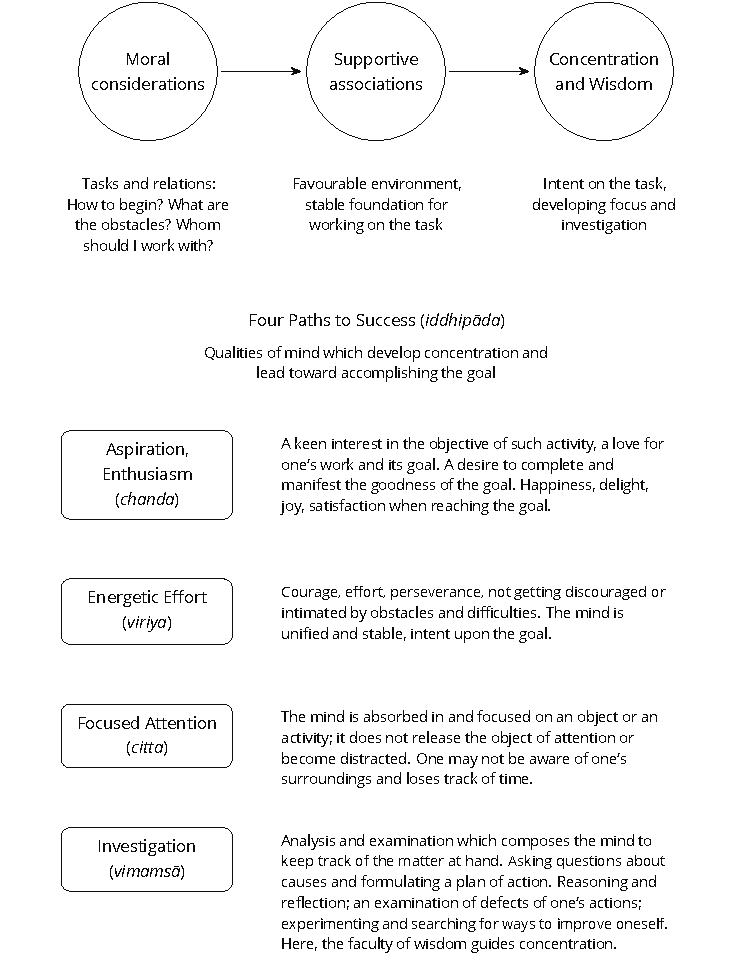
\includegraphics[width=0.95\linewidth]{./manuscript/tex/diagrams/paths-to-success.pdf}
\end{figure}

\clearpage
\normalpagelayout

Quiet and peaceful times are a blessing. I always appreciate a stable
routine which allows for long periods of concentrated work or dedicated
practice. That said, obstacles and conflicts are guaranteed to arise.

We don't have to worry that meditation is going to solve our every
problem and that we will have nothing left to do. Meditation is not
problem-solving. It is a practice of awareness which overcomes inner
obstacles and faces external problems as they arise. If we have
something important to do, it helps to clear our head first. But merely
sitting on a cushion as if we have transcended all problems, we are
practising ignorance the present, not the awareness of it.

Voluntarily facing obstacles and addressing them skilfully is a golden
chance to develop the mind beyond our preconceived limits. The confused
chaos is rich in the potential to develop and learn in a practical way.

We are not seeking the feeling themselves, not trying to create special
feelings by meditating, or seeking the ideal situation where everything
will pleasantly work for us. Pleasant, unpleasant, neutral feelings will
not, in themselves, give us right understanding if we follow their
influence and react mechanically. Awareness has to notice their
impermanence and uncertainty. With this, we can see what is wholesome
and what is unwholesome in the present situation.

\enlargethispage*{\baselineskip}

\keywords{boat moving on the river, me and mine}

Is meditation practice easy or difficult? A useful image to think about
is how a boat moves on a river. When the boat is packed and burdened
with product-filled crates, it moves heavily and slowly. It is just
barely holding itself above the water.

We want our boat to go fast, don't we? But at the same time, we are
holding onto everything we packed it with. We have to lighten our boat,
and let go of the heavy burden of the self. We create the burden of `me'
and `mine'. We create the impression of `I have been like this. I am
like this. I should be like this.' `That was mine. This is mine. This, I
want to keep. That, I have to get'. This is the weight that is holding
our boat down.

The sense of having enough creates the mental space for generosity.
Contentment is an ongoing part of practice. It is not a fixed state
attached to conditions. Wise action and learning flow like a stream from
contentment: When I think, `I will be ready to do it when I have
\ldots{}', discontent occupies my thoughts and keeps interrupting my
focus on the current situation.

\keywords{wholesome thoughts, peace}

But when I think, `I am not good at it, but I have enough to start',
accepting my current limits gives me energy for action. Then I often end
up doing more than what I thought.

Thinking has a bad reputation in meditation texts, but clear thoughts
create a condition for developing right attitude. Proliferative,
compulsive thinking is a painful experience, but wanting to stop all
thinking also misses the target.

Notice how wholesome thoughts are followed by contentment and peace.
Consciously recollecting one's moral actions establishes a sense of
stability and self-respect. We can trust ourselves to let go of the
superfluous because we feel we already have enough.

If we try to solve it in our head, the practice is going to get
complicated fast. In meditation, awareness through the body is a
reliable guide: Watching the feelings and mind states as they come and
go, we shift our view from being preoccupied with ourselves. We can
leave behind complicated questions because we no longer need the
answers.

\keywords{light boat, enjoyable learning}

What enables us to keep learning and developing? The journey is most
enjoyable when the horizon keeps expanding beyond our previous limits.
We expand the horizon not by travelling far, but by seeing with new
eyes. The desire to hold onto what we think we are creates our current
limits.

The boat is light, when it is empty of me and mine. It can cover great
distances without making drama and fuss. What happens, if we are sitting
in a boat, and somebody runs into us with their boat? We shout at them,
push them away with the oars, and complain about it for the rest of the
day. All this might be justified, but we ruined our day with our own bad
company. It's hard to see the wisdom in that. What happens if an empty
boat floats into our boat? Where did the earlier anger and negative
emotion come from?

We tend to manufacture stories about me and mine, whether based on real
or imagined events. If we take them seriously, and give them reality,
the stories start to control us, and we create problems which didn't
exist before.

\enlargethispage*{\baselineskip}

Sometimes we sit on a meditation cushion and start playing out inner
arguments with puppets of the imagination. It's a serious business! We
have to win! Methodically thinking through a problem is a powerful tool,
but sympathy and kindness toward ourselves is necessary for a
constructive inner dialogue. Otherwise, when the self is talking with
itself, it finds itself in bad company.

\keywords{he who can laugh at himself}

It's surprising how we can wind ourselves up about a situation which
hasn't even happened yet. It helps to keep a pinch of humour in our
side-pocket in case of emergency seriousness. Recollecting a saying of
the Greek philosopher Epictetus, `He who can laugh at himself never runs
out of things to laugh at.'

\keywords{simplicity of the senses, letting go}

In the practice of meditation, we restore right view by returning to the
simplicity of the senses. If stories arise, we observe them from the
perspective of changing conditions. By investigating the senses, we take
a more fundamental level as our basis for attention. Pleasant feeling is
like this, as we are experiencing it. Unpleasant feeling is like this.
Neutral feeling is like this. They have a beginning and an end, they are
changing and empty.

In the practice, the value comes not in accumulating results in a hurry,
but in leaving space for letting go and patience. There are times for
action, but simple patience solves a surprising variety of difficulties.
The sense of being hurt, the feelings of urgency and importance come
from ourselves. Restraint gives us a safe perspective, guarding
ourselves and others. Let us allow our boat to move on in silence.

\chapter{Bones}

\keywords{physical pain during meditation}

\noindent Even if we are sitting in good posture, sooner or later,
something somewhere is going to hurt. Practising in a good posture
minimizes unnecessary discomfort, but it can't eliminate it entirely.
Pain and discomfort comes with the fact of having a body, but we are not
meditating to torture ourselves, and we can take care to avoid injury.

Regarding pain in the body, we can either investigate it as a meditation
object, pay attention to another area of the body where there is no
pain, or change our posture.

If our habitual reaction to pain is a sense of anxiety, aversion and
restlessness, then a period of investigation can be useful. Remember the
intention that you wishing yourself well. Then investigate, observe the
pain, how it shifts around in the body, how it arises and ceases in
waves. `Who is suffering? Is it changing? Where is the awareness which
knows this?' This changes our perception from experiencing pain as an
emergency situation which needs to be solved right now, to experiencing
it as a signal which we can choose to put aside for a time.

\enlargethispage*{\baselineskip}

The pain may not be a sign of injury, like, for instance, the discomfort
comparable to what we feel sitting through a long bus ride. We might
choose to keep our attention on a different part of the body. Or we can
move our attention methodically around the body, noticing a spot where
it is not painful, and meditating while staying with the sensations in
that area.

An interesting exercise is to locate exactly where the edges of the
painful area are. Is it a sharp or diffuse boundary? Does it stays
fixed, or does it gradually shift around? This investigation
familiarizes us with the arising and ceasing nature of the pain. It
becomes less of a big deal. We don't have to react with aversion to it,
there can be some free space for the unpleasant sensations to just be.

When you do decide to move, before you move, pause for a moment and
establish a clear intention: `I move out of compassion for the body. I
change posture because I wish my body to be well and healthy.' Then
shift your legs or change posture. This keeps the continuity of
mindfulness intact as we are not then reacting out of aversion or
restlessness.

\keywords{contemplating the body, bones, perception of self}

\enlargethispage*{2\baselineskip}

After a sitting session, you might change the posture to standing, and
allow the joints and the muscles of the body to relax. Standing requires
more attention to maintain balance, and the bones -- the supporting
structures of the body -- are easier to feel.

The bones make up the core, the rigid parts of the body which determine
its shape and what it can and cannot do. Without bones, our body would
be a blob of meat. With bones, it has an inner structure which gives it
the outward appearance we are familiar with. We look in the mirror and
think, `that's me'. How thoroughly did we examine the image before
seeing ourselves in it? A brief glimpse of its outline, contour and
colour will already trigger the perception of `me'. We have a fairly
static image of ourselves, in the present we remember ourselves as an
image from several years ago. Since the rate of change is slow, we rely
on fewer and fewer key features to recognize the image in the mirror.

\clearpage
\thispagestyle{empty}\mbox{}
\photoFullBleedPlaceholder{%
  TODO: Illustration of standing meditation.%
  \illustration{Standing Meditation Posture}%
  \label{illus-standing-meditation}%
}
\clearpage

Leaning closer, noticing more features, or seeing ourselves from an
unusual angle, it might take minutes to decide who we are looking at.
What determines this image? If the bones were slightly different, the
body would be a different shape. Such a change would change not only our
appearance, but also how we live.

\keywords{standing meditation, standing posture}

Stand in an upright but flexible manner and take some time to find your
balance. Place the feet at shoulder width, with the knees relaxed and
slightly bent, being engaged in holding the body. Don't let the knee
joints lock up straight. This stresses them and will cause your posture
to become rigid. Keep the feet parallel, with the toes pointing straight
ahead. Rotate the hip toward the front along the horizontal axis,
slightly pulling in the lower half. It is a motion like turning a bucket
with the open top turning toward oneself.

Sway the body left and right a bit and feel the centre of weight.
Develop a sense that you are holding the body upright, that you are
preventing it from falling. It is better to balance the weight of the
body toward the heels, rather than leaning on the balls of the feet.

Hold the shoulders wide enough to open the chest for easy breathing, but
not so wide that they become tense. A comfortable place for the hands
can be for example on the thighs, at about over the place where the
pockets are on a pair of jeans.

Allow yourself some flexibility and make small adjustments to your
posture as your muscles get used to the situation. Feel out your balance
in standing and watch, take notice of the body as you hold it this way.
Gravity is pulling it down. There is pressure on the ground. If that's
better, let your hands rest in front of the abdomen, one palm
comfortably on the other.

The eyes may be open or closed. If you feel drowsy, you might prefer
meditating with eyes open, but keep your gaze lowered, looking only a
couple of meters in front of you. If you look straight ahead, your
attention will be directed outwards, and various movements such as those
seen out a window will be distracting.

If you close your eyes but it feels strained and painful, pay attention
to where the eyes are focused when you close them. If they narrow in
close, as if focusing on something close behind the eyelids, this causes
the inner muscles of the eyes to strain and dry. This tension and
dryness can even cause the eyes to water up with tears.

On traditional Buddha statues, the eyes are depicted as being slightly
open. He is awake, not sleeping. Instead of shutting your eyelids tight,
practise relaxing them. Let them stay lowered without any pressure.
Though your eyelids are mostly shut, imagine looking at something far in
distance. This lets the eye muscles relax. To allow some light in, you
can try allowing a narrow slit to remain open. It can also help to
massage the inner eye muscles a bit with the tips of the thumbs in a
circular motion.

Breathe in, and watch how your posture changes with the movement of the
breath. The diaphragm muscle pulls in the air and the abdomen moves
forward to give way. The shoulder bones rise, the ribs in the chest open
outwards, and your body's centre of gravity shifts slightly.

\enlargethispage*{\baselineskip}

Is there something limiting the breathing? Take care to stand upright
and don't let the shoulders hunch as this blocks the open breathing.

Take note of the balance of the head and find the position where the
head sits on top of the spine of its own weight, not leaning forward or
pulled backward. Instead of looking directly ahead, direct your gaze
slightly down in front of you, so as to mitigate your attention becoming
distracted by any comings and goings. Pulling in the chin, direct your
gaze a couple of meters in front of you on the floor. Allow the crown of
your head to rise up a bit, as if pushing the sky.

The position of the head controls the posture of the upper body to a
great degree. Through years of sitting on chairs, we have developed the
habit of pushing our heads forward which creates tension in the back
muscles along the spine. Although we can't control these muscles
consciously, we can experiment. What does it feel like to pull the head
back a bit? You can feel out the balance where the muscles in the back
relax.

In a balanced posture, the vertebrae of the spine sit one on top of
another, like carefully positioned stones. With the spine aligned
upright, gravity is enough to keep it settled in place. Such a posture
gives us a pleasant feeling of light balance without forcing.

\keywords{attitude to the body, analytical mind, goodwill}

If our attitude is too analytical, it can conjure up grotesque and
shocking impressions of the body, but a sense of goodwill towards
ourselves can keep the meditation balanced and wholesome.

The intellect functions by building abstractions and separating out what
it observes. When viewing the body, it might see the various parts as
abstract and inanimate objects. Keep in mind that we are not practising
body-contemplation to create aversion or alienation to the body. We are
practising meditation with clear comprehension in order to see things in
their context, nothing is isolated in a vacuum. Our body-awareness
includes rather than excludes and must come from a welcoming attitude of
acceptance and goodwill.

This difference of attitude reminds me of a story about a dialogue
between Plato and Diogenes. Plato was giving a lecture to his students
at the Academy in Athens, where he defined men as `featherless bipeds'.
Diogenes happened to overhear this and, being fond of practical jokes,
he brought a plucked chicken to Plato and held it up in front of him
proclaiming, `Behold! I've brought you a man.' He must have thought that
this would show that a certain context was lacking in Plato's overly
intellectual definition.

The group at the Academy added `\ldots{} with broad flat nails' to the
definition, in an attempt to satisfy their scholastic sensibilities, but
probably still missing Diogenes' point.

\keywords{experiencing the whole body}

We watch the sensations in the body as we breath in and as we breath
out. Turn attention inwards, mindful of the perception `the body is like
this'. The mind is not seeking, not going off around the world
somewhere. It does not need anything, what is here is enough. Awareness
sees the body, from the feet, to the legs, abdomen, chest, arms,
shoulders, the neck and the head. The body is one whole, one changing
perception, sensitive to the breathing.

\enlargethispage*{\baselineskip}

Watching the body like this is like watching the rain. There is nothing
to do, nothing to decide. The rain just goes on without us having to get
involved.

\clearpage

\keywords{clear comprehension, awareness of the body, defusing anger and desire}

Unskilful thoughts are comparable to dust blowing in the wind: it blocks
our vision, we can't see anything from them. The Buddha compared the
effect of awareness on the mind to rain, as it settles the dust and
clears the air. `Quelling such {[}unskilful{]} thoughts and
considerations, like rain on the dust, with a heart calmed of thought,
you'll touch the state of peace right here.'\footnote{\href{https://suttacentral.net/iti87/en/sujato}{Iti
  87}, Destroyers of Sight}

Awareness of the mind stops unwholesome mind states from arising,
develops wholesome mind states, this way purifying the heart. We may
notice that our experience of the world is not fixed: we are not
isolated outside observers, looking onto a world which is separate from
us. We have a part in creating the world we experience, since we form
its impressions through our mode of attention.

When clear comprehension is established and you notice the mind becoming
more clear and stable, review what allowed this change? What did you do?
What did you \emph{not} do? You didn't have to fight or manipulate the
sense experience or the thoughts and emotions, since they change through
the change in the mode of attention.

Our mode of attention creates the frame of reference from which we
experience the world of the senses, dependent on perception and memory.
This is a process that conditions a certain attitude, like a function
operating over time, which produces how we recognize and interpret
ourselves in the present.

\clearpage

Shifting our mode of attention can serve to stop providing unwholesome
mind states with more fuel. From the perspective of direct experience,
and in accord with the way things are, such unwholesome states are then
denied a basis or reference for their continuance.

In brief, we can say that awareness of the mind purifies the mind.

Staying with the awareness of body defuses both anger and desire. It
changes the frame of our attention and such mind states then fall flat
as though the carpet had been pulled out from under them. The busy,
thinking mind is like a noisy show, or the news in last year's paper.
The topic is no longer interesting, it has lost its urgency, it keeps
going around the same circles. Put the thinking down, like a weary hiker
their heavy backpack, and continue mindful awareness of the body.

Periodic distractions and daydreams can occur, but keep returning to the
breath and the physical sensations of standing. If while standing, you
begin story-telling or fantasizing until the bell rings, that's not
practising insight meditation\ldots{} it is practising waiting for the
bus.

\keywords{memory as self, narratives of self}

\enlargethispage{\baselineskip}

Investigate your state of mind as an experience. The perception of your
body and its feelings arise before we construct the perception of self
from it. What do we remember about ourselves? If we forget about the
narrative that someone told us yesterday, or if we recollect being with
friends years ago, do we perceive ourselves differently?

This interaction between our memories, feelings and mind states keeps
changing. Current perceptions keep changing, and recognizing awareness
places trust in a place which knows this change. This allows us to see
from a wider frame, where there is no fear of the change. Creating the
perception of our self is an ongoing process. We take an active part in
it through actively recalling and re-creating memories. We narrate a
story of ourselves from the memories of the past, and choose choose what
to do now.

\keywords{bones, parts of the body, sense of inadequacy, judgements of appearance}

Observing the body and its parts, our minds stay with the changing
perceptions before the creation of a self. This process disarms the
self-judgement, fears and expectations that bog us down.

Notice the feeling of how the bones connect. There is this perception of
an inner structure which supports the body from the inside: rigid
pieces, connecting end to end, and stacked on top of each other. There
are sensations in the legs: rigid perceptions denoting the long leg
bones. There is pressure. The hip bone is resting on top of the legs and
the torso moves joined above all this. The rib-cage expands and
contracts with the breathing. The spine is holding the weight in a
curve. The head is sitting on top of the spine. The skull bones are
stretching the skin of the face.

\enlargethispage*{\baselineskip}

Our body is made up of pieces. In some places, these pieces are hard and
rigid. In others, they are soft and flexible. The combination of these
is what gives our body its shape. When we look at a person, all we see
is hair of the head, hear of the body, nails, teeth and skin. And we
then construct a person from it all. We glance at a mirror for a
fraction of a second, recognize the general outline or notice some
particular feature, and think, `That's me. How do I look?'

\clearpage

\enlargethispage*{3\baselineskip}

\begin{figure}[h]
\caption{Experience and Illusion of Self}\label{fig-illusion-of-self}

\centering

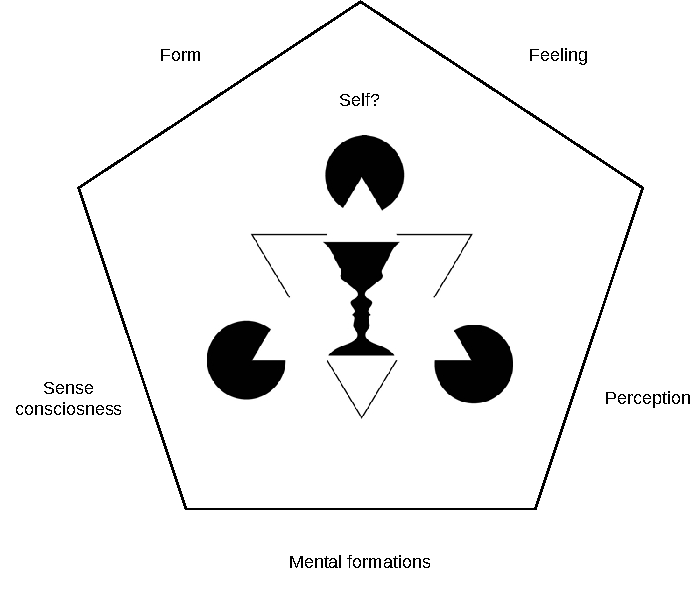
\includegraphics[width=80mm]{khandhas-self-illusion.pdf}

\bigskip

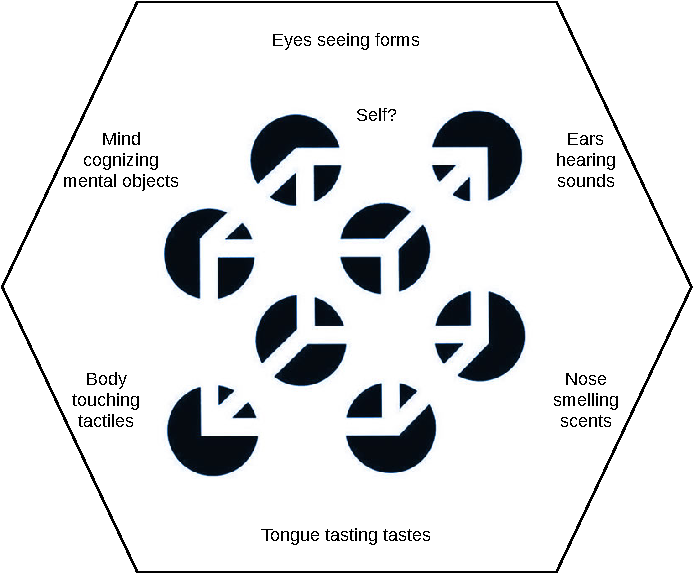
\includegraphics[width=80mm]{senses-self-illusion.pdf}

\bigskip

{\small
We experience a self, which has no substance beyond that experience.
Above, conditioned expectations create filled-in shapes which we \emph{experience}, but are not there.
The Kanizsa Triangle, Rubin's Vase and Subjective Necker Cube are examples of illusory contours.
}

\end{figure}

\clearpage

In some situations, we can notice the gradual steps of how this
perception builds up as when we see someone walking in the fog. First,
we recognize the shape of a `person'. Then we detect `male' or `female'.
Maybe it is someone we know? Some detail triggers the final recognition
of our friend and their name. This entire process plays out in the realm
of perception.

The habitual perception of the body -- both of our own body and of other
people's bodies -- is that we see it as one unit, one thing. From that
perspective develops an obsession that there is some ideal way that it
should be. We imagine that the body has to be a certain shape, a certain
size, and so on.

These are worldly judgements, perceptions which our society has drilled
into us. Some cultures idealize a thin body, others a plump one, and
these cultural ideals keep changing from one generation to the next.
Advertisements and various messages from the media reinforce these
expectations and we dutifully believe in them. When we look closer, we
see that such perceptions are twisted and not in accord with reality.

We can be very concerned about what other people think about us, but how
much are \emph{we} concerned about the appearance of others? If I watch
myself, I don't think much about how other people look. But I can feel
self-conscious and imagine that \emph{they} must be thinking about
\emph{me}. When, in fact, they think about me as much as I do of them --
not much, if at all. They are occupied with getting on with their own
life, just as I am with mine.

Besides the pressure of our self-judgment, we imagine how others are
judging us. And since we can't know and can't control what they think,
we internally ruminate in the mind about it, which creates an illusion
of such knowledge and control. When we play out these inner dialogues,
we enjoy the illusion of control. But we miss out on the freedom of
letting go of \emph{the need} for that control.

\keywords{body parts as not-self}

We can notice the conditioned nature of this anxiety when various parts
of the body become detached. We can be so concerned about our hair, for
example\ldots{} but only when it is on our head. When the hairdresser
cuts it off, we are not anxious about the pile of hair on the floor.
Similarly, when cutting our nails, what is that point when it is no
longer `me' and `mine'?

When we contemplate the body in this way, we see it not as one unit, but
as made up of pieces and parts which have their own nature and behave
accordingly, each part not the least concerned with our opinions or
those of others. Bones, skin, hair, teeth and nails: they are the way
they are.

The body is a blessing. This meditation is not meant to develop aversion
toward the body. Health is a blessing, it supports us in everything we
do. The Buddha called health the greatest treasure.

\keywords{stories as dreams, awareness of the body, grey and drifting states, gratitude}

We observe the breath, the parts of the body, and our present
experience. When we look, we find that they don't carry the stories of
`me' and `mine' with them. Since it is we who are creating these
stories, we can also stop creating them, we are not chained to following
them. Phenomena arise through dependent conditions. When the conditions
cease, the phenomena cease. This is all that happens.

Awareness of the body loosens the grip of our desires and leads us to
recognize that we are fortunate to be here. We can always return to this
attention: one in-breath and out-breath is enough to remember arising
and ceasing. Doubts become like stories in an old newspaper. We get
tired of untangling the threads of the past which are so difficult to
follow. It is like interpreting someone else's dreams.

What is real, is always here in our present experience. What becomes
important is not who or what we are in the story, but whether we can
give our attention to where we are now.

Clear intention has an important role. When we don't set a clear
intention, we are drifting. Perhaps we don't particularly mind being
here and drifting like this, but the mind is grey with no life, almost
trying to hide itself and be invisible. We end up being grey and
invisible like that. Nothing wrong is happening, but there isn't any
brightness and joy in being here.

We don't stop often enough to notice when we are happy and peaceful.
When the mind is clear and calm, the natural feeling is a sense of
gratitude for what is here, and for the blessings we have received in
our life.

\enlargethispage*{\baselineskip}

Gratitude is not created by will. In this practice we are not creating
anything, we simply recognize what is here with clear intention. It is
not a matter of strength or ability as those are bound to time and
circumstance. But resolution and mindful attention are not bound to a
given circumstance. The result is a right perspective in which we can
see the right order of things and what to do with them -- or to stop,
give attention and breathe.

\chapter{Awful}

\section{A Constructed Image}

\keywords{superficial impressions, bitterness, false expectations}

\noindent -- Hello, how are you feeling today?\\
-- Awful.

This is not what a meditator is supposed to say, is it? They should
respond positively, such as, `I'm feeling great, it's such a lovely
day!' Or at least `I'm OK, and how are you?' We have an image of a
`meditator' in our heads who is supposed to behave and speak in certain
ways, while not behaving and speaking in certain other ways. We might
ask, `Who has put that image in \emph{my} head?'

The image of the `good meditator' is a perception formed from
superficial impressions which, without deeper examination, we have
allowed ourselves to see as real. Imagine opening an article about
meditation. (While continuing to read the current one\ldots)

\enlargethispage*{\baselineskip}

It starts with the smiling photo of a monk or a lay meditation teacher,
and it continues by describing the positive effects of mindfulness. It
might include stories and photos taken at a retreat. People are sitting
on meditation cushions with serene faces while the light through the
window is illuminating the Buddha statue. The article might contain
interview excerpts about how participants had overcome their inner
struggles. It ends with the encouraging words of a meditation teacher,
or with a quote from the Buddha. THE END.

Even someone not terribly interested in meditation knows what this
article looks like, we have seen dozens of them. There is no need to
include a reference source, the chapters in this book could be examples
as well.

This is not to suggest they are being deceitful. The authors write with
good intentions. They are trying to encourage us to continue on the path
of contemplation and to put effort into our practice. If we can't see a
greater happiness beyond the frustrations, what would be the point? If
there was only suffering and misery to expect, we don't need help in
creating that.

\keywords{happiness, get out of your own way, removing blocks from a river, vipassana-glamour}

Buddhism is fundamentally optimistic, and one of its central theme is
happiness. Our typical attitude is that we seek the things which give us
happiness, or that want to create the circumstances necessary for our
happiness. But it is not sure that we understand the right attitude, and
we can become so entangled in seeking happiness, that we become more and
more bitter, as it can seem that such happiness can never be realized.
We assume the fault is in our circumstances or personal abilities, but
in reality the problem is that we don't understand how things work, and
this is why our attitude leads us in the wrong direction.

Our task is not to search for happiness, but to understand the cause
which gives rise to suffering, and stop creating it. Through
understanding this, happiness spontaneously appears in the mind.

Our way of thinking is like continuing to keep carving a statue until it
is \emph{just right}, but with which we are never satisfied. We think
it's our fault, and we don't notice that the materials of the statue are
just the way they are. The clay, sand and stone will remain what they
are. The groups of \emph{khandhas} -- form, feeling, perception, mental
conditions, and consciousness -- will remain as they are. What creates
the struggle is when we expect them to be otherwise.

Effort is necessary, but a more useful metaphor for wise practice could
be that of a choked up river: when boulders of stone are obstructing the
flow of the water, creating turbulence. We tend to focus on the
turbulences of our feelings, and while trying to stop the vortices, we
create more of them. It may be the case that all it needed was to remove
the boulder blocking the flow: let's not grasp the whole shebang as `I
am this'. Sometimes we just need to get out of our own way.

If you observe the water flow in a river channel, you'll notice vortices
forming behind obstacles. Their back-and-forth motion might seem
familiar (see Figure \ref{fig-grasping-turbulence}). When holding onto
the perspective of `I am' dominates the mind, we start flipping
back-and-forth between opposites. We reason with ourselves what to do
because `I like A', or `I don't like B', `I should do X', `I shouldn't
do Y'.

Not satisfied with either, but holding onto an identity, the mind is
stuck in a flip-flop between the extremes. One opposite invites the
other as a reaction, the extreme positions being easier to reach, rather
than a cool-headed look at the situation from an outside perspective.

The teachings do mention suffering frequently, but such instruction is
given on the ground that freedom from that suffering is possible. The
Buddha made it clear that the fruit of the path is genuine happiness,
and if it was not possible to practise it, i.e. to abandon unwholesome
roots and develop the wholesome ones, he would not have taught~it.\footnote{\href{https://suttacentral.net/an2.11-20/en/thanissaro}{AN 2.19}, Skillful}

Who is that meditator in our head? One thing is sure, the one in
\emph{my head} is always a \emph{better meditator} than I am. When
someone takes a good photo of us, we know how it is: it was a good
moment when we looked orderly or even glamorous, but we know that in
five minutes the opposite could be true. And although this is true not
just for us, somehow we don't remember this about good photos taken of
other people.

These are a sort of \emph{vipassana}-glamour shots -- it's a bit vain
but we like looking at them. They make good illustrations in an article,
but we should remember that the same people will look different in an
ordinary moment.

\clearpage
\figurepagelayout
\null\vfill

\vspace*{-4\baselineskip}

\begin{figure}[h]
\caption{Grasping and Turbulence in the Mind}\label{fig-grasping-turbulence}

\hspace*{-2.5mm}%
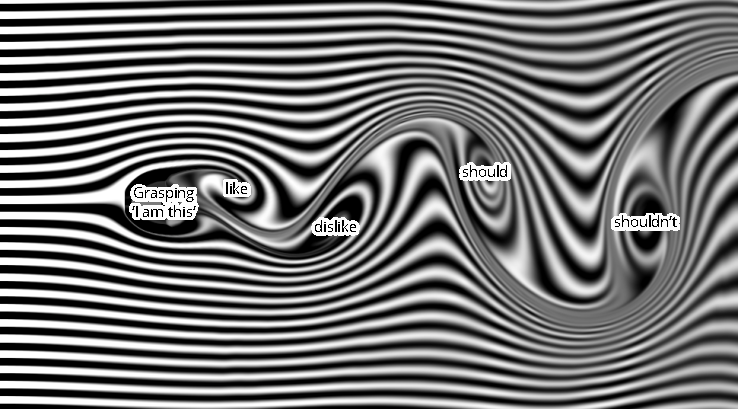
\includegraphics[width=\linewidth]{./manuscript/tex/diagrams/grasping-turbulence.pdf}

\bigskip

\hspace*{10mm}%
\begin{minipage}{\linewidth-20mm}
\footnotesize
Turbulence in obstructed water flow.
The formation of vortices is similar to how grasping 'I am' in the mind
causes one to be stuck in a back-and-forth motion between opposite positions.
Fluid simulation by Amanda Ghassaei (\href{http://apps.amandaghassaei.com/VortexShedding/}{apps.amandaghassaei.com}).
\end{minipage}

\end{figure}

\vfill\null
\clearpage
\normalpagelayout

\section{Threads}

\keywords{suttas as literature}

\noindent In the days of the Buddha, one form of literature was the
\emph{sutta}, which means a thread of discourse. \emph{Suttas} may
include prose and verse, and were intended to be memorized through
recitation. The community of monks would compose a \emph{sutta} after a
significant event, such as a discussion or formal a teaching, to give
the story a formal presentation in which they would memorize it. The
Buddha certainly encouraged them to do so:

\begin{quote}
Thus you should train yourselves: `We will listen when discourses that
are words of the Tathāgata---deep, deep in their meaning, transcendent,
connected with emptiness---are being recited. We will lend ear, will set
our hearts on knowing them, will regard these teachings as worth
grasping \& mastering.'

\bigskip

\quoteRef{%

\href{https://www.dhammatalks.org/suttas/SN/SN20_7.html}{SN 20.7}, The
Peg

}
\end{quote}

Today, books, articles and blog posts fulfil a similar function, to
distribute curated information. These modern media, when bringing their
best form, hold up the canonical \emph{suttas} as their example. The
monks of the early years delivered their message to us through these
threads, and their efforts have become part of our conversation with
those we meet today, just as our written works will speak to those in
the future who we will never meet.

\clearpage

\vspace*{-\baselineskip}

\keywords{social media, selection bias, Instagram Effect}

In today's social media the clear understanding of the message is
distorted by what is called `the Instagram effect', which is a selection
bias to show only our best and most positive side, and filter out the
negative one, which is nonetheless just as real and necessary for
complete understanding.

This influence is not negligible. Medical studies have already started
discussing a related form of depression and obsessive behaviour called
`Snapchat Dysmorphia'.\footnote{\href{https://www.ncbi.nlm.nih.gov/pmc/articles/PMC5933578/}{Is
  ``Snapchat Dysmorphia'' a Real Issue? (ncbi.nlm.nih.gov)}} In these
cases a given person seeks cosmetic surgery to look more like the
smiling photos they see in the application.

The automatic filters of the app edit every picture to be more
attractive, and if we repeatedly see our bodies shown to us (by the
application) as a nearly flawless image, \emph{that} becomes our mental
self-image, and the unfiltered image we see in the mirror seems wrong to
us.

One might consider a similar Instagram Effect in published articles
about meditation experiences. The author has a point to explain, and
they select a mix of personal experiences, opinions, and supporting
explanations from other authors.

The author may write truthfully and try to avoid selection bias, but
subtle, unconscious forms of self-filtering keep operating. The world of
the written text is always a constructed reality. Nonetheless, when it
succeeds in its goal, in the well-chosen words we recognize our own
experience.

\clearpage

\vspace*{-\baselineskip}

\keywords{our mental images as role models}

The meditator who lives in our head is like a character in a poem, or
the hero in a myth. Our heroes are wiser and stronger than we are, so
that when we are feeling lost and weak, they can give us faith and
advice. They can have unshakeable peace, so that when we are feeling
awful, we are able to endure and wait until the difficulty ends.

Such mental images are, however, just that, and shouldn't be mistaken
for a real person. They are valuable sources for guiding ourselves,
their narrative description helps us to figure out what to do by showing
where we are in a bigger picture.

The role of a mental image is not to determine what we \emph{should
become}. When we relate to perceptions and ideals like that, we are
going to feel conflicted and inadequate, because the real circumstances
of our life are far more complex, rich with ambiguous, shifting
boundaries, and are not like the simplified, static reality of a mental
image. Mental images are tools for explanation. They are \emph{ways of
seeing} the world, and are examples of acting correctly in a given type
of world.

\clearpage

\section{Assumptions}

\keywords{mind and the world, mode of attention, actions and beliefs}

\noindent We may remember the verse in the Dhammapada which points out
that the world of our experiences is not independent of us:

\begin{quote}
Mind precedes all states of being: they are led by the mind, made by the
mind.

\quoteRef{%

\href{https://suttacentral.net/dhp1-20/pli/ms}{Dhp 1}

}
\end{quote}

Does that mean that we are creating imaginary problems for ourselves?

We may start investigating by asking, `Can the subject experience
suffering?' Living beings can suffer, but a cultural idea or self-made
story cannot suffer, even while \emph{we are}. It changes our attitude
if the subject of our concern only exists as a story and not as a living
being. Such insentient stories include the narratives we have around
institutions, nations, money, fame, or other social fabrications.

Next, a quick moral safety test: `Would a wise person praise or
criticize doing this?'

Further on, bringing our view to the surface: `What assumption creates
this stress and pressure? What is the motivation for doing this? Without
what, would this have no significance?'

We can reveal such unconscious motivations by looking at our present
actions and choices. What we choose to do now expresses what we believe
in, the assumptions we have accepted in the past.

`Why am I choosing to do this, here? Where does this action come from
and where does it lead?'

The underlying factors for our actions may come, for example, from the
habitual conditioning of our environment. We may have not expressed in
thought why we do what we do, but have felt \emph{the results being
expressed on us}, whether good or bad.

Starting the investigation with a closer look at our actions and
\emph{then} asking about the thoughts motivating them is a productive
method. In our inner chit-chat we tell all sorts of contradictory things
to ourselves, but our actions give clear points of reference.

\keywords{the best place to learn, reversing assumptions}

The associated feeling might be awful, but if we treat it as sign to
turn toward the mind and investigate it, our approach will stay
practical and productive. `If I am here anyway, what can I learn from
this?'

We find access to our assumptions through uncovering our unconscious
motivations. Once we can express an assumption clearly, we gain the
freedom to reverse it, or drop it.

We may ask, `Does it help in this situation, if I reverse my
assumptions?' Perhaps looking at it in the opposite way is exactly what
is we needed either for peace of mind, or for dropping the issue as if
it never existed. Either way, we are not acting out of compulsion: we
are free to either let it go or \emph{choose} to follow it through.

\clearpage

\section{After the Storm}

\keywords{happiness and accomplishments}

\noindent Meditation guides say, `return to the present moment', but it
doesn't mean that you must like everything you find there. The point is
that this is the only place where you can live. If you are happy, you
are not happy in the future, but in the present. If you are suffering,
you can't understand it in the future, only in the present. In some
situations, no amount of brainy self-talk is going to make it better, it
is best to call it the way it is, and wait out the storm like a stoic.
Conflict is genuinely stressful, separation from what we love is sad,
and being alive always ends with the tragedy of our own death.

We tend to anticipate success, and we expect our hard work to be
justified in the future. Examine that moment of accomplishment, what do
you experience? There may be some emotional elevation -- surprise, joy,
exhilaration, relief -- then everything is back to the ordinary level.
The destination turns out not to be the deliverance we thought it would
be. If we were intensely focused to get there, we might not even
remember anything from the journey, and wonder where did all the time
go. We can be so intent on being productive, that we waste our chance to
live.

Contemplating death holds up a truthful, if somewhat scary, mirror to
our values. `If I were to die tonight, would I be happy to remember
living as I am living today?' This question can stir up more from the
deep recesses of the psyche than we wish for. I remember a time when my
response the word `happy' was exclusively anger and self-aversion.

\clearpage

\vspace*{-\baselineskip}

\keywords{values, being busy, Hedonic Treadmill, burnout, contentment}

The term `Hedonic Treadmill' describes the adaptive process in which
each new achievement becomes the new norm in our psyche, and we feel
less and less emotional impact after succeeding at our goals. Like on a
treadmill, no matter how hard one tries to increase one's happiness by
pushing toward the next successful step, one still remains in the same
place. We spend our life travelling on the journey, not hanging out in
the destination. If we look closer, even the idea of any destination
evaporates, like when you fly into a cloud. `I thought I saw it right
ahead, but now that I'm here, I can't see it.'

Despite this, we seem to continue thinking that being busy, productive
and efficient, is somehow going to save us. When one project is
finished, we can feel that we \emph{need} another one because being busy
is the only way of existence we know.

The wise men of old repeat their message about contentment, but it seems
that we have to suffer the pain of burnout before we comprehend what the
problem is.

Bertrand Russell gives a diagnoses, `One of the symptoms of an
approaching nervous breakdown is the belief that one's work is terribly
important.'\footnote{\href{https://www.goodreads.com/book/show/51783.The_Conquest_of_Happiness}{The
    Conquest of Happiness by Bertrand Russell}}

Henry D. Thoreau writes in
his cabin by Walden Pond, `It is hard to have a Southern overseer; it is
worse to have a Northern one; but worst of all when you are the
slave-driver of yourself.'\footnote{\href{https://www.goodreads.com/book/show/16902.Walden}{Walden
  by Henry David Thoreau}}

\clearpage
\figurepagelayout

\begin{figure}[h]
\vspace*{-15pt}
\caption{Achievements and the Hedonic Tredmill}\label{fig-hedonic-treadmill}

\centering

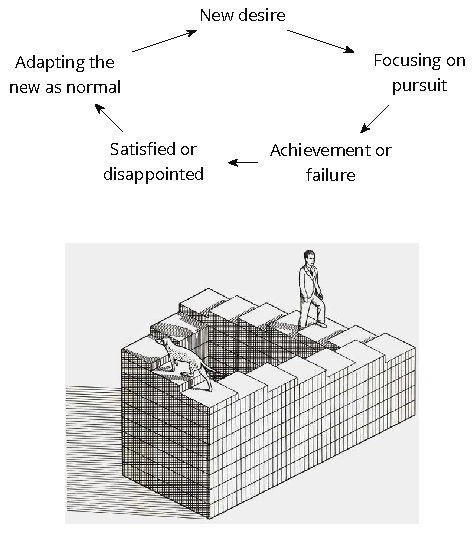
\includegraphics[width=90mm]{./manuscript/tex/diagrams/hedonic-treadmill-stairs.pdf}

\bigskip

\begin{minipage}{0.8\linewidth}
\centering\footnotesize

The Hedonic Treadmill is the tendency for new achievements to be adopted as a modified, \emph{normal} baseline,
and for our level of happiness to return to the same level as before.
After one desire is satisfied, the conditioned craving seeks a new state.

\bigskip

The person on the Penrose Stairs thinks that
they are getting further and higher.
From our outside perspective,
we see that they are merely returning to the same level as before.

\bigskip

Recall the definition of Noble Truth of the Origin of Suffering:
`It is this craving which leads to renewed existence,
 accompanied by delight and lust, seeking delight here and there;
 that is, craving for sensual pleasures, craving for existence,
 craving for extermination.'
(\href{https://suttacentral.net/sn56.11/en/bodhi}{SN 56.11})

\end{minipage}

\end{figure}

\clearpage
\normalpagelayout

What if you practice \emph{being free}, instead of practising \emph{to
become free}? The system of gradual training described by the Buddha --
while encouraging us to make diligent effort in our practice -- starts
with blameless happiness in the present, born of contentment through
moral- and sense-restraint.

\begin{quote}
{[}\ldots{]} they practice restraint, protecting the faculty of mind,
and achieving its restraint. When they have this noble sense restraint,
they experience an unsullied bliss inside themselves.

\bigskip

\quoteRef{%

\href{https://suttacentral.net/mn38}{MN 38}, The Longer Discourse on the
Ending of Craving

}
\end{quote}

\keywords{self-aversion, self-criticism, labyrinth of mirrors}

It is easy to over-correct being busy, and swing to the other extreme:
`I've had enough! I'm just going to quit everything!' This might seem
``logical'' but, being driven by aversion, we continue to suffer. For
many of us, it is easy to be critical of ourselves, and we diligently
practice it with conviction to prove ourselves wrong, as if
self-aversion was a virtue.

`I am feeling awful! A \emph{real} meditator would never feel like this.
I must be doing something wrong.' A whole identity can be built around
this, a ceaseless internal monologue which always responds with
complaints and self-aversion. One can live like this for decades, and it
becomes the baseline by which we recognize ourself. `If I wasn't feeling
angry, I wouldn't even know who I was.'

It is like being stuck in a labyrinth of mirrors: everywhere you look,
you only see yourself. The key to escape is to find a crack in the
mirrors, and recognize change: the feelings of being driven, and the
motivations of anxiety and anger which we thought were constant are, in
reality, changing all the time -- breaking up and reforming. This
labyrinth has been made by the mind, and what it has created is empty of
self. It cannot be what we truly are.

Doubtless, we can find a persuasive logic in our self-defeating
ideations, and our reasoning for being critical can be completely
reasonable! Psychologists say that the most difficult patients are the
ones who intelligently defend and justify their own bad habits. We can
be so clever that there is absolutely no way to be happy \ldots{} and we
can prove it! Can you recall ever playing the role of such a miserable
philosopher?

But we do not necessarily experience immediate relief when our
self-reflection reveals to us the emptiness of what we have been
pursuing. Anger, despair\footnote{The Buddha compares dealing with anger
  and despair to walking along a path close to a deep drop-off.
  (\href{https://suttacentral.net/sn22.84}{SN 22.84}, With Tissa)} and
sadness can be our first reaction, generating thoughts of self-aversion.
We purify the mind with the mind: These mind states are not reliable,
they shut down our intelligence, and who wants that? So we let go.

\keywords{patient endurance, gratitude, no hurry}

Patient endurance is an underappreciated virtue, but often, all we need
is to remember to wait: the dramatic rain and thunder of turbulent
mental states will run themselves out.

When the sense of gratitude appears, it is a sign like the rainbow after
a storm. It accompanies wholesome mental states, and we can
intelligently see the situation from more than one angle. This is a good
base from which we can build useful thoughts about what to do next.
Sometimes, the best thing to do is to simplify and turn away from
certain habits and values. Other times, our view has changed and we
might wish to keep up what we have been doing, but leaving the big hurry
behind. We continue for the sake of living it, not waiting for some kind
of elevated mental state in the future.

\begin{quote}
One should not revive the past\\
Nor speculate on what's to come;\\
The past is left behind,\\
The future is unrealized.

\bigskip

\quoteRef{%

\href{https://suttacentral.net/mn131}{MN 131}, One Fine Night

}
\end{quote}

\section{Humour and Irony}

\keywords{opinions, changing perspectives, noticing what is pleasant}

\noindent There are morose, dark moods which are like sand-traps of
logic, made by ourselves. The more we think about them, the deeper we
sink in them.

Humour and irony are funny because they show the situation from
unexpected and odd angles. If the logical path straight ahead is
blocked, why not try the sideways track where the fox goes? A joke
wouldn't be funny if it was logical and reasonable. Humour and irony,
directed toward ourselves, are good friends when it seems that we can't
escape the suffering of our thoughts.

What makes the old and wise men \emph{wise}? Medical studies\footnote{\href{https://www.researchgate.net/publication/258190619_Aging_irony_and_wisdom_On_the_narrative_psychology_of_later_life}{Aging,
  irony, and wisdom, William Randall (researchgate.net)}} have
investigated the various attitudes of senior citizens, and found that an
inclination toward self-directed humour and irony (i.e. being able to
laugh at oneself) was helpful to face the significant challenges of
ageing and maintain mental balance and a positive outlook on life.

One of their key observations is that humour and irony develop our
ability to see ourselves from multiple viewpoints. We can fill the role
of the accurate historian and the jesting comedian at the same time.
Hence we are able to see events from multiple narrative angles and not
be caught in a single story. The frame of the narrative we see ourselves
in remains open as we move toward a positive future. The limits of our
being don't necessarily mean the end of the story, and we don't have to
go far to find good laugh: in the absurd corners of life, there is
always a joke to tell.

It can be rude to joke about somebody else's bad situation, but who is
going to get upset over your humorous comments about yourself? If you
feel awful, how about an awful joke? This trip is so bad that it's good,
and the tickets are free. `What am I? An animated skeleton in a skin-bag
with clothes on, standing here with a fabulous hair-cut, and I can prove
the logic of \emph{my important} opinions.' What's not to laugh at?

We say that in meditation we observe our own mental habits, but
sometimes we practise this with a critical bias: we observe the
\emph{bad mental habits}, while we don't notice the good ones. It is
possible to become so good at ignoring pleasant mind states that one
genuinely believes happiness only exists for other people. When
something good happens and you feel happy, stop and notice it, `Hey,
this is nice.' This increases our capacity to recognize and experience
such mental states in the future. Who will notice it if you don't?

\section{Expectations}

\keywords{symbol of Buddha statues, changing predictions, relinquishment}

\noindent We might look at a Buddha statue and expect ourself to
meditate in the same perfect posture without moving, like the Buddha.
But in this case we have missed the message of the statue, which points
to inner qualities rather than external signs.

A Buddha statue is not a depiction of the historical \emph{Siddhattha
Gotama} Buddha who lived in the 5th century BC. We don't have a statue
of him made during his lifetime. We know from the \emph{suttas} that he
was normal height and good-looking, but instructed the monks to not
focus on his physical appearance, bot on the Dhamma, the truths of the
mind instead.

He taught them that even if a monk were grabbing hold of the corner of
his robe, but if they didn't see the Dhamma, they would not see the
Buddha.\footnote{\href{https://suttacentral.net/iti92}{Iti 92}, The
  Corner of the Cloak} The first Buddha statues were made four or five
hundred years after his death by Greeks in the Gandhara region of
Afghanistan. Buddha statues represent the wisdom and serenity of the
awakened mind, expressed in the human form.

They are beautiful to look at, but nobody is going to become a Buddha
statue, just like you can't become the photo of the perfect meditator,
or the hero in lyric poem. They do offer advice, but the advice can't
orient us when taken rigidly. We should apply the advice by taking our
inner experience and the present situation into account. This way we
return to the awareness which awakens to the truth and overcomes
obstacles. The practice of virtue, and the trust in the examples of
skilful teachers is a strong foundation. We can wish ourselves well,
while still admitting that we feel awful, when that's how it is.

Expectations are a prediction of the expected value of a result, they
estimate the outcome of our situation. Meanwhile, every factor which
goes into that prediction is changing. We have to allow the prediction
to change, our expectations of our mental experience must keep changing
according to where we are now. Having expectations is not a problem, but
if we attach to a particular outcome which we believe to be `the real
one', this becomes a hindrance. It turns out that if we invest in future
emotional states as the basis for our happiness, the result will be
disappointment.

\enlargethispage*{\baselineskip}

The \emph{ānāpānasati} breathing technique taught by the Buddha has
sixteen steps. The first is knowing whether the breath is long or short.
But what is the last step? We might wonder, `What could be that exalted
mind state which we will reach?' Mindfulness meditation on the
breathing, after contemplation of the body, feelings, and mental states,
follows contemplating the natural truths, of which the last step is:

\begin{quote}
One trains thus: `I shall breathe in contemplating relinquishment'. One
trains thus: `I shall breathe out contemplating relinquishment'.

\bigskip

\quoteRef{%

\href{https://suttacentral.net/mn118}{MN 118}, Mindfulness of Breathing

}
\end{quote}

The practice of the Eightfold Noble Path is not about accumulating, but
about transforming our values through insight into the experience of
changing conditions. At the end we relinquish the conditions, like
putting down a burden and not carrying it any further. This includes all
that we take to be `me and mine'. Anyway, how long can we really hold
onto anything?

\keywords{real practitioner, Impostor Syndrome}

Reflection and cultivation opens up a wider field of view where
opposites can exist in complex relationships. In the contrasting
approach, we exalt the judgmental and comparing mind, and this limits
our scope. Such a perspective wants to sort things into neat, mutually
exclusive abstract categories, which leads to mistrust and harm. We
start losing faith, not believing ourselves to be `real' practitioners,
and others don't seem to be credible ones either. The result is that we
can't learn from ourselves, and we can't accept anyone to teach us
either. This doubt is blinding and paralysing, it feels like we can't do
anything. The problem is that our expectations are too narrowly focused.

\enlargethispage*{\baselineskip}

It's not that there are no problems and difficulties. Explaining to
ourselves that `pain is not painful' is not a meditation technique
taught by the Buddha. But we shouldn't assume that we should be like
mythological ideals. Meditation is not a button to control mental
states. It is cultivating awareness, so that mental states don't control~us.

\section{Calibrating Emotions}

\keywords{learning emotions, variation is the norm, disappointment, saññā and saṅkhāra}

\noindent When we talk about emotions to each other, we often explain
their mechanism roughly as a `neural circuit', or a region in the brain
which gets activated in a certain situation. According to this story,
some brain areas are wired from birth to produce given emotions, and
they make us feel fear, love, anger or disgust.

But then how do we explain it when a person without an \emph{amygdala}
still experiences fear? The \emph{amygdala} is typically seen
responsible for that emotion.

Or how about more refined categories?

The Japanese `\emph{mono no aware}' means a sadness over transience and
the beauty found in that, are the Japanese born with such a neural
circuit? By the description, you might recognize the feeling, if you
have seen Japanese movies it might even be familiar, and now, fitting a
verbal expression on it, it gets easier and easier to feel it.

Other cultures find the western emotions strange, for example the Utka
Eskimos, who have no direct equivalent of the concept of `anger.' Or the
Tahitians, who have no concept of `sadness.'

Medical research informs us that no particular emotion has a built-in
`brain-circuit' from birth.\footnote{\href{https://www.goodreads.com/book/show/23719305-how-emotions-are-made}{How
  Emotions Are Made: The Secret Life of the Brain by Lisa Feldman
  Barrett}, Theory of Constructed Emotion} It is not the given emotion
that is fundamental, but our ability to recognize patterns of loss and
reward, to \emph{learn emotion concepts} from other people, and to
recognize them in a new situation in the future.

In any given situation, the brain recognizes if an earlier experience
\emph{in a similar context like this} was rewarding or not. This becomes
easier over time if we have learnt to associate an emotion concept with
it, becoming a spontaneously automatic feeling.

The instances of an emotion category are variable: `fear of a tiger' is
different from `fear of an exam', which are learned and adaptive
predictions. They fit only to some extent, like a person may fit a
stereotype, but no person is a 100\% example of every feature of the
stereotype.

Our brain evaluates the present based on the past, and according to
whether good or bad can be expected, there is a response we feel
throughout the body, and we construct an instance an emotion from it
based on our concepts.

\keywords{emotions are categories, not distinct mental object, learning emotions, what is wrong with me}

In the classical model of emotion -- which we are accustomed to in
everyday discussion -- we treat emotions as distinct mental objects. The
idea is that an emotion has clear attributes that any two mentally
healthy people should agree on.

However, while they were studying the brain in action, it became
apparent to the scientists that this cannot be the case. As they
conducted more and more studies, the evidence continued to contradict
this view.

When people undertook physical and psychological tests about the
emotions they experienced, the results had great variation between
individuals. There were no universally distinct, clear markers, or
`fingerprints' to identify any given emotion. Rather, the
\emph{variation was the norm} in both people's emotional experiences,
the meaning and function of those emotions, and their corresponding
physical reactions.

The scientists found that our body and brain \emph{learns} emotion
categories through a process of conditioning perceptions. From our
culture, the other people we live with (socially conditioned emotions);
from biological needs (bodily conditioned \textasciitilde); or from our
personal history, such as long-time habits, significant events and our
memories.

This also relates to how one person might not understand, or not even
recognize, the emotions of another. For example think of the culture
shock when visiting a distant country: an emotion such as `love' has a
variety of expressions, contexts and underlying assumptions which were
not part of our earlier emotion category of `love'. It can take a while
to pick up the new signs and meanings until we can feel the subtle
differences, and we can reliably recognize the signs in others.

Ask yourself, how do you know that you are feeling a particular emotion
such as \emph{metta} (loving-kindness) or \emph{sukha} (happiness)? The
model we use for our understanding of emotions influences what we expect
to happen in our meditation practice. If we think of emotions as
distinct things, as though they were external objects which we wish to
reproduce, or have access to, then we can easily feel `this is not it, I
don't know what's wrong with me'.

Since \emph{variation is the norm}, our experience will probably differ
from other people's. Individual meditation experiences are as varied as
the individuals. A given instance of an emotion can be expected to vary
from the generalized idea. It is important to rely on knowing \emph{our}
mind states and feelings, instead of trying to reproduce external
descriptions.

Our freedom extends to learning and constructing emotions we never heard
of before. We rely on mindfulness to perceive our experience, we
self-train the concept, and establish the conditions for the emotion to
arise.

Using the terms of the Five Khandhas, we would say that perceptions
(\emph{saññā}) and mental conditioning (\emph{saṅkhāra}) influence each
other and establish patterns of experiences, which we learn to identify
as a present instance of a broader, abstract emotion category.

We start with reading the external description and we turn it into an
inner experience through reflection and daily actions. Knowing our
experience is the reference point. Over time, the new experiences become
familiar to us and they arise without effort.

\keywords{emotions as predictions, culture shock, adjusting expectations}

The brain is constantly receiving signals from the nervous system, and
based on what it has learned, it tries to predict whether the present
situation is going to mean energy input or energy expense for the body.

The brain responds by preparing your body, such as increasing or
decreasing the heart rate, starting or stopping the production of
certain hormones. We experience this bodily reaction, and if earlier we
learnt an emotion category which suits this, we feel an instance of that
emotion: fear of danger, excitement in anticipation of immediate reward,
or euphoric happiness.

This explains culture shock: if you have grown up in a different
culture, you've learnt different emotion categories, and when travelling
to a distant country, the emotional world of the people living there can
be unfamiliar to you.

We tend to believe that our experience is like the view when we look out
a window. One `looks onto their experience', and sees what is going on.

It turns out that the picture is rather more incomplete than we think,
when we take into consideration how the senses and the nervous system
work. The brain doesn't have much information to work with, so it has to
guess at what is happening from simple signals, hints about what the
rich world outside of itself might be like.

The brain can't see much: it's sitting in the skull, which is, in
effect, just a dark box. Bodily fluids, chemicals and nerve signals
carry messages into this box. The messages come from other systems in
the body, which are themselves noisy and sometimes conflict with each
other. From this clutter, the brain has to generate a perception of the
place where we are, guess what is happening to us, predict what is
likely to happen in the next minute or so, and produce a response which
is hopefully going to help us survive, or even lead to happiness. It has
to do all this, from inside a dark box, based on a few noisy and limited
signals.

What am I then? An animated skeleton, and my head is a dark box? Well,
that does explain a lot of confusion. Is it a wonder that my predictions
are a bit off, and need constant adjusting? What I experience as reality
is ongoing guesswork, changing by the second.

\clearpage

`Happiness equals reality minus expectations' -- a memorable phrase by
Tom Magliozzi. These days, our expectations are so high. We receive
updates from social media apps, we read web articles, and each time they
influence our view of how we are, and how the world is around us. They
show us perfect, determined, or outrageous images of other people. Since
we don't meet these people face-to-face, we don't see the real
background of their lives, and this exaggerates our expectations. It
trains the brain again and again to expect these artificial
presentations, like an expectation machine on overdrive. We don't even
notice the distorted self-conditioning, but we are disappointed and
exhausted, which leads to ceaseless dissatisfaction.

\keywords{simplicity, impermanence, self-reflection, values}

We have the ability to calibrate the `expectation machine' through the
balancing effect of conscious reflection and reasoning. `What is the
most important today? What do I need for this one day?' When you
simplify the answer down to the essentials, it's not that much. Food,
clothes, shelter, medicine, supportive companions and perhaps something
to do toward a worthwhile goal.

The average day is probably more messy, and doesn't hold to this
abstract, pure simplicity, but this exercise is only for recognizing the
baseline. If simple is enough, then it won't be a problem to be able to
do more, or have access to more, while contentment remains our baseline.
Ambition is not the problem, but hyping up our expectations blocks its
application.

Expectations are necessary to follow a given direction in the world, but
not understanding them, they become obstructions in the heart.
Expectations and emotions are of the nature to arise, twist, flip-flop
and then turn around. Let them pass on by, like leaves in the water next
to a boat. Bad ones are not that bad and good ones are not that sure.
Knowing their changing nature, we don't take them so seriously and don't
get stuck on them, as a boat shouldn't get stuck on some leaves.

\begin{quote}
Whether it be pleasant or painful\\
Along with the neutral,\\
Either internal or external,\\
Whatever feeling there is:\\
Knowing them, `This is suffering,\\
deceitful and disintegrating,'\\
Coming in contact again and again,\\
seeing their fall,\\
One loses one's passion for them.

\bigskip

\quoteRef{%

\href{https://suttacentral.net/sn36.2}{SN 36.2}, Pleasure

}
\end{quote}

\clearpage

\section{Happiness as Flourishing}

\keywords{meanings of happiness, results, day-by-day practice, death, contentment}

\noindent Our modern Western culture often presents happiness as a
particular feeling, or as a certain circumstance in life which we are
supposed to arrive at. We pass on our culture through discussion with
one another. Our way of talking about happiness tends to treat it as an
outcome, as an event in the future, or as a certain state of being. This
seems to be a recently developed trend, and not necessarily a helpful~one.

Traditionally, we view the ancient Greeks as one of the most influential
societies in the formation of our Western values. Aristotle (384-322 BC)
is one of these influential thinkers, and today we are still reading and
referencing his writings which survived the ages. In these texts, he
investigates the question of happiness in great detail.\footnote{\href{https://plato.stanford.edu/entries/aristotle-ethics/}{Aristotle's
  Ethics (plato.stanford.edu)}} He was concerned with what happiness
was, and with how to live a happy life, but, unlike us moderns, he did
not see it as a particular result or circumstance.

The Greek word he used for happiness is \emph{eudaimonia}, and can be
translated as `human flourishing, prosperity.' He saw it as
an active process which we practice day by day, rather than
an eventual outcome in the future. He describes the practice of
happiness as being based on moral virtue and a truthful view of one's
life from birth, growing up, old age, and including the tragedy of one's
own death.

\enlargethispage*{2\baselineskip}

This direct view of virtue and mortality puts things in order: it gives
us a wide perspective in which happiness is founded in wholesome mental
qualities, and we look beyond ourselves to give lasting meaning to it.

Training our expectations in this way, the practice of happiness is a
complete whole every day. We learn to be with the struggle when that's
how it is, applying our best abilities in virtuous ways, and at the end
of each day, we can look back with contentment.

If the field of `happiness research' in psychology, Daniel Kahneman and
his team have conducted interviews asking people to recall the episodes
of the previous day and to later answer questions about them.\footnote{\href{https://www.goodreads.com/book/show/11468377-thinking-fast-and-slow}{Thinking,
  Fast and Slow by Daniel Kahneman}, Day Reconstruction Method} The
evaluation confirmed that attention and recurring thoughts are the
dominant factors in whether one feels happy or depressed. While the
volunteers were going through a variety of everyday situations, how they
felt was determined not by where they were and what they were doing, but
by what they were thinking about at the time.

\keywords{deathbed regrets, life as a unit of time, hierarchy of needs, self-actualization, self-transcendence}

\enlargethispage*{3\baselineskip}

But it surprised them to find that when people spoke about what kind of
day they had, they didn't talk about happiness as a good feeling, but
rather they reflected on social experiences, friends and relatives, who
they met and what they did together, and on whether they felt satisfied
with their life or not.

All this makes sense when we examine our experience: the perspective,
the frame through which we see the world orients us, while the content
of the frame continues to change. The hungry person sees the world in
terms of food, and where to get it. A person in an ambitious mood
focuses on `what I can do' and `how good I am'. A person considering the
limited time of his personal existence, tends to turn toward values
which are self-transcendent. Rather than focusing on experiences created
by the self, one turns to timeless qualities apparent here and now.

It was a discovery for me when I was listening to an
interview,\footnote{\href{https://www.samharris.org/podcasts/making-sense-episodes/209-a-good-life}{A
  Good Life: A Conversation with Scott Barry Kaufman}} and heard the
psychologists discuss a new addition to Abraham Maslow's hierarchy of
needs. This is usually pictured as a pyramid starting with the need for
food and water at the bottom, and ending with self-actualization
elevated to the pinnacle. This seemed to be a rather ego-centric way of
thinking about happiness.

The psychologists recently re-discovered Maslow's late
writings,\footnote{\href{https://bigthink.com/neuropsych/maslow-self-transcendence/}{Maslow's
  forgotten pinnacle: Self-transcendence (bigthink.com)}} and found that
toward the end of his life, he felt conflicted about his system of the
hierarchy of values: he was going to die, fundamental parts of his needs
(e.g. survival) were lacking, hence he should be miserable, but instead,
he felt relief and states happiness which he called `peak experiences':

\begin{quote}
Feelings of limitless horizons opening up to the vision, the feeling of
being simultaneously more powerful and also more helpless than one ever
was before, the feeling of great ecstasy and wonder and awe, the loss of
placing in time and space with, finally, the conviction that something
extremely important and valuable had happened, so that the subject is to
some extent transformed and strengthened even in his daily life by such
experiences.
\end{quote}

\clearpage
\figurepagelayout

\begin{figure}[h]
\vspace*{-15pt}
\caption{Hierarchy of Needs, Self-Transcendental Values}\label{fig-self-transcendental}
\bigskip
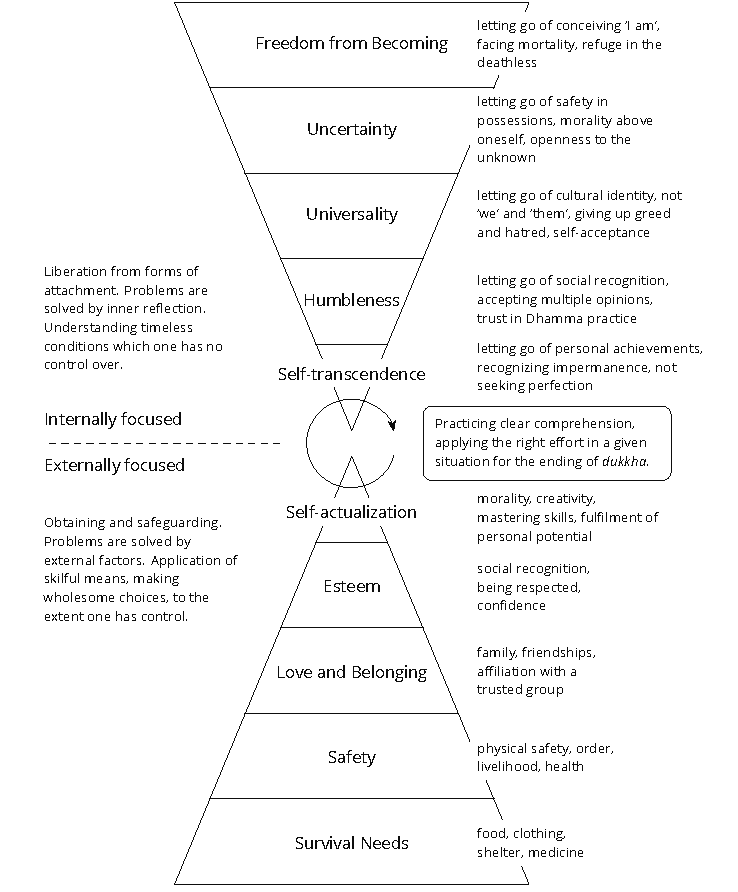
\includegraphics[width=\linewidth]{./manuscript/tex/diagrams/self-transcendental-values.pdf}
\end{figure}

\clearpage
\normalpagelayout

Maslow appended another level to his hierarchy of needs above
self-actualization: \emph{self-transcendence}. Examples include: not
holding onto perfection, not fixating on one's opinions, giving up the
need for certainty, giving up the attachment to one's past and letting
go of the fear of death.

`Self-transcendence' sounds like something for a Buddha, but since we
are suffering from our attachments to one thing or another, it turns out
to be a basic \emph{need} for all of us.

Holding onto what we think we are creates the very limits which we
struggle with. We want to expand our horizon but we are held back by
grasping an identity. When that identity turns out to be an empty void,
we urgently need help. Think of the day-to-day struggles: being
conflicted over opinions, stressed out about our abilities, anxious due
to unexpected changes, lamenting past tragedies. A self-transcendent
perspective is necessary to get over ourself.

Still, we do keep the score on how things are going for us, don't we?
Wholesome conditions are our supports. This is the time and place where
we live, not any other: \emph{memento vivere}, remember to live. We know
if our efforts are aligned with our core values or not, even though we
can get distracted with things we didn't intend to spend so much time
on.

I remember how it shook me up when I read in a description by a
nurse,\footnote{\href{https://bronnieware.com/blog/regrets-of-the-dying/}{Regrets
  of the Dying (bronnieware.com)}} that some of the most common deathbed
regrets included working too hard and losing touch with old friends.
Life is a unit of time with a beginning and an end, and we should treat
it as such.

\keywords{\emph{memento mori}, \emph{memento vivere}, \emph{amor fati}, \emph{saṃvega}, \emph{pasāda}}

If tuning the mind to a comfortable numbness is `tranquillizing
ourselves with the trivial',\footnote{A phrase used by Søren Kierkegaard
  in The Sickness Unto Death} then recollecting death (\emph{memento
mori}) is a dose of anti-tranquillizer. Since the time is limited, we
recollect the urgency to live (\emph{memento vivere}) and do what must
be done before it's too late. This motivates us to find the courage to
be true to ourselves and turn toward the situation we are living in
(\emph{amor fati}), not waiting for some place and time we imagine in
the future. In the Pali language of the Buddhist \emph{suttas},
\emph{saṃvega} refers to the sense of spiritual urgency, while
\emph{pasāda} expresses the serenity of having confidence in the Path
and its practice.

Reading about deathbed regrets was a timely reminder for me to think
about the urgency I felt about completing projects (which come and go by
the month), and not losing the opportunity of spending quality time with
long-time companions.

Reflecting on life as a single unit of time includes being born, growing
up, growing old and dying. Remembering our mortality this way puts our
values back in line with the facts of nature. We can give ourselves some
time to dwell where we are, and appreciate it before it's over. We seem
to understand the fleeting nature of good and bad feelings when we
compare them to the importance of our golden relationships.

Remember that we wish ourself well-being and happiness, and that we wish
our family and friends happiness in their life. Consciously recollecting
moral virtues builds mental resilience and self-respect. We can
acknowledge ourselves: `That was a good thing to do. I've done that
well.' Or, we see it in others, such as in teachers, role models, and
friends.

It develops gladness and appreciation of what is good in other people as
we share in their successes. There is a wellspring of happiness in
cultivating the face-to-face companionship of friends whom with we
mutually feel glad at our successes in life. We can use humour to ease
up a bad mood, and complete the next step forward.

The present is change itself. We bring that experience into awareness
and contemplate the body, feelings, mind states and natural truths
following the refrain in the \emph{Satipaṭṭhāna Sutta}:

\begin{quote}
\ldots{} One dwells contemplating its nature of arising, or one dwells
contemplating its nature of ceasing, or one dwells contemplating its
nature of both arising and ceasing. \ldots{} And one dwells independent,
not clinging to anything in the world.

\bigskip

\quoteRef{%

\href{https://suttacentral.net/mn10}{MN 10}, Mindfulness Meditation

}
\end{quote}

\chapter{Why}

\section{Doubt and Faith}

\keywords{compulsive thoughts, orientation of views, unexpected changes}

\noindent Sometimes we are interested in meditation in order to deal
with a disturbing or painful experience. We know something is wrong and
we can't shake it off. Or it could be a sense of feeling lost, where
nothing makes sense: such feelings keep returning, they don't let
themselves be ignored. Instead of answers, only the questions keep going
round and round: `Why does it have to be like this? What should I do,
and why? What's the point?'

Even in such confusion, merely acknowledging the state of our inner
chaos to ourselves already starts to provide some order and orientation.

\enlargethispage*{\baselineskip}

It is like driving on a road cluttered with trash. Slowing down to look
around is already much better than being blind to the dangerous clutter.
Our head is full of thoughts but only a few of them indicate reliable
directions, so we better examine them. Previously, we held a view that
things in our world were one way, but they have changed in a way we
didn't expect. It is not their fault, it is not our fault, but the
unexpected change is confusing, and we have to adjust our view.

Impermanence pulls the carpet out from under our feet, but at the same
time transforms our values, the qualities which we seek out as valuable
in our experiences. If we don't understand the change, it causes
confusion, followed by doubt. Even though we might know what we
\emph{should be doing}, we get stuck in the sense of doubt and
meaninglessness and we can't even begin.

\keywords{meaning, investigating what I believe, faith as fuel}

Why do you get up in the morning to do anything? Why does it matter at
all? If I keep asking `why' and dig into the layers of my constructed
self like this, the first layer reveals a matter of habit, `because this
is what I did yesterday'. Under that, the answers are formed out of
stories I tell myself about myself and the world I live in. Under that,
there is some degree of reasoning, philosophy and abstract ideas. Under
that, I am desperately trying to hold onto something solid, and I start
defending my ideas with personal memories and experiences (`because when
I was like this and this \ldots{}'), or I refer to famous names
(`because this and that teacher said \ldots{}').

Under that, I have to give up and confess that it is a matter of faith
and personal conviction. What I do is simply what I decide there and
then. At the end, I stand there and have to admit that I don't
\emph{know}, but I \emph{believe} that doing such-and-such makes sense.

Faith is not a fixed quality in the mind. We have the capacity to choose
credible statements which we perceive will guide us toward a greater
understanding and happiness. We can test any given belief by applying it
in practice and by observing the results, and we can then support or
abandon that belief accordingly.

I may review, investigate and update \emph{what I believe} about what
makes sense to me, but until my experience verifies it, my reasoning has
to be supported by faith. Otherwise, I will not make an effort in any
direction, and my life will be governed by blind habits and external
pressures.

Faith is the fuel for the virtues of resolve and energy. Later on, faith
will be reinforced by experiencing the results of practice, but without
fuel, our car doesn't even start.

\keywords{belief as a cause of action, trust in the teacher}

A belief creates a cause for an action. Without that belief, I don't
take that action. In the Buddhist perspective, there are two fundamental
beliefs:

\begin{enumerate}
\item
  A phenomena occurs when the sufficient causes for it are present; and
  it either does not occur, or it ceases, when the sufficient causes are
  absent.\footnote{\href{https://www.dhammatalks.org/suttas/SN/SN12_61.html}{SN
    12.61}, Uninstructed}
\item
  The Buddha completely understood the truth about the way things are,
  and thus freed himself from greed, hatred and delusion. Hence he is an
  excellent teacher of the way of practice.
\end{enumerate}

The Buddha gave us the instruction that each person should question,
ponder, and investigate the way things really are to understand it for
themselves. Nonetheless, how are we going to start? Without trust in the
teacher, we are lost in the tangle of our personal opinions and it is
unlikely that we are going to listen and learn anything new. The
tradition reminds us of this relation to faith when, before giving a
Dhamma talk, we start by chanting \emph{namo tassa} three times.

\begin{quote}
\emph{Namo tassa bhagavato arahato sammā-sambuddhassa}

Homage to the Blessed, Noble, and Perfectly Enlightened One.
\end{quote}

\keywords{doubt, wandering in a desert, grasping creates limits}

The Buddha compared doubt to being lost in a desert, wandering around
without water.\footnote{\href{https://suttacentral.net/dn2}{DN 2}, The
  Fruits of the Ascetic Life} Everything else is secondary: we can only
think about how to find water and escape the desert.

Or, we fantasize about how to comfortably numb the mind and not think
about anything at all, `tranquillizing oneself with the
trivial'\footnote{Søren Kierkegaard, `The Sickness Unto Death'} to
continue everything as normal. In doubt, it is not clear how we will
escape this situation, but we can start by acknowledging the aspiration
to be well and to live a happy life.

It is our natural human ability to overcome confusion and develop
long-term happiness in our lives. A long-term view has to include
changes to our situation, loss and tragedy. Stable happiness has to be
founded on a perspective which integrates impermanence.

In the \emph{suttas}, doubt appears both in the list of Five Hindrances,
and in the first three of the Ten Fetters, which are the ones that
obscure understanding the Four Noble Truths. When doubt gets personal,
there is no doubt that it leads to suffering. Figures
\ref{fig-leading-to-suffering} and \ref{fig-leading-to-cessation}
illustrate how we get into this mess, and how we can get out of it.

As a hindrance, doubt stops Right Effort, and stops developing the mind.
As a fetter, it compels us to keep looking for fixed certainties, and
thus ties us even tighter to our ideas about who we are.

We like the suggestion to develop our mind, but initially, we think this
means making sure who and what we are, getting more of what we need, or
changing ourselves to become something different.

`Who am I? What am I? What should I do? Is this the right thing? Or is
it something else?' This way of thinking is a trap, it goes round and
round with no way out. All these concerns are tied up with holding onto
some kind of identity which will again invite doubt. Until we realize
what is happening, we are caught in the cycle.

Even when we become successful, at the end of that becoming, it is going
to change according to its nature, and we find that our new identity is
also hollow, empty of real value, just as our previous idea of ourself.

Grasping at and holding onto what we think we are, being afraid to let
go: this is the obstruction. This creates the very limit we are
frustratedly running up against. Understanding freedom through letting
go doesn't come to us easily.

\cleartoverso
\figurepagelayout

\begin{figure}[h]
\vspace*{-10mm}%
\caption{Leading to Suffering}\label{fig-leading-to-suffering}

\centering

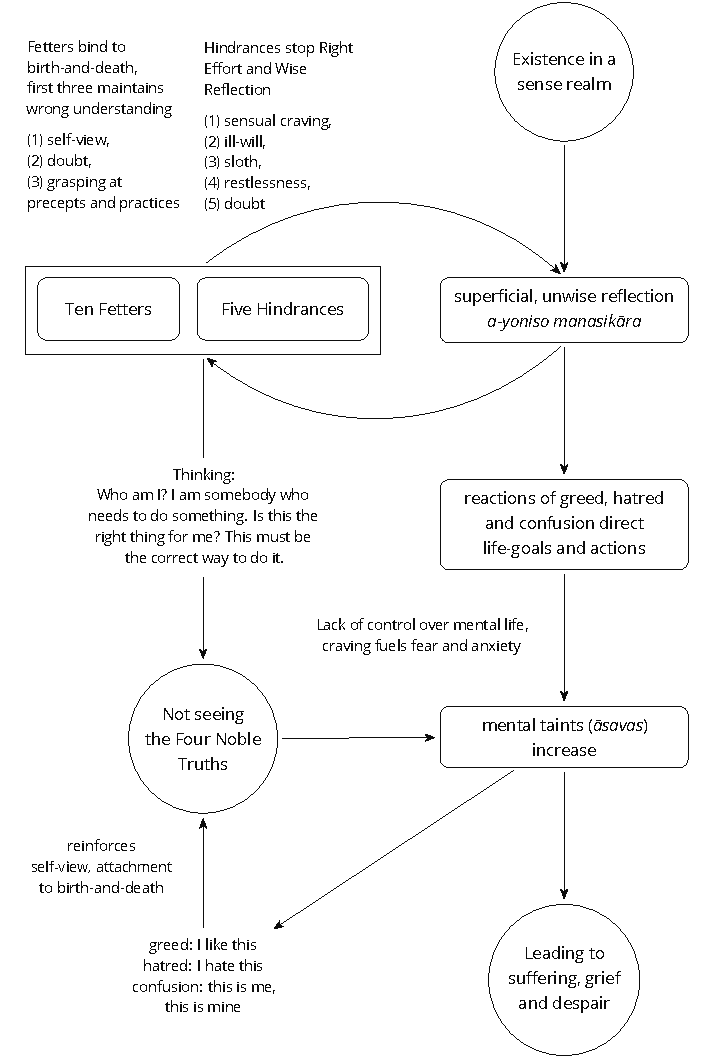
\includegraphics[width=\linewidth]{./manuscript/tex/diagrams/leading-to-suffering.pdf}

\end{figure}

\clearpage

\begin{figure}[h]
\vspace*{-10mm}%
\caption{Leading to Cessation}\label{fig-leading-to-cessation}

\centering

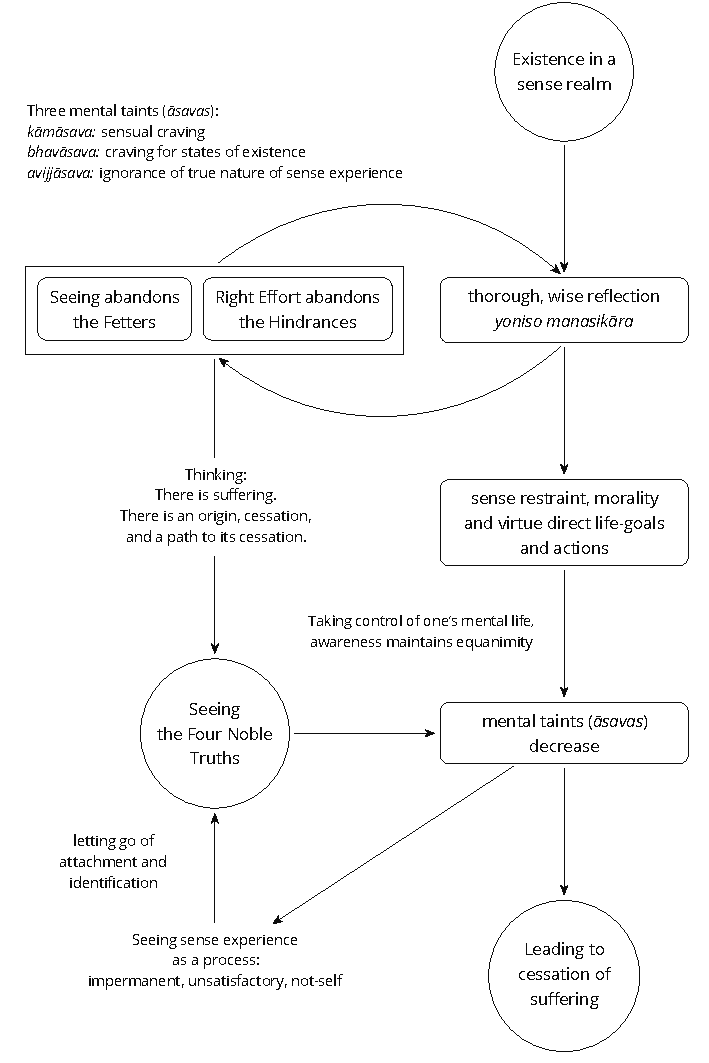
\includegraphics[width=\linewidth]{./manuscript/tex/diagrams/leading-to-cessation.pdf}

\end{figure}

\clearpage
\normalpagelayout

\section{Right View}

\keywords{returning to the beginning, observing thoughts}

\noindent Let's return to the breath and continue the meditation
practice. At the beginning of a session, start with the basics, simple
steps which guide the attention back to the familiar frame: the in- and
out breath, the body and its feelings. Observe what you are experiencing
as a process which is going through continuos change from one feeling
into another.

Every meditation session is a new beginning, we can't save the results
of the previous session and load in the knowledge. If we start thinking
we already know, say, if we have been practising this for years, this
results in a closed attitude which blocks even our earlier
understanding. Our experience from the past is only relevant when we
apply it to the present. The changing present keeps understanding fresh
and new.

`This thought, this feeling had a beginning, it is changing now, it will
cease and end. Can I wait and notice that cessation?' Contemplating
direct experience this way, the mind gives up its desire and fear
regarding particular states, and understands them as part of natural
processes. We are not reasoning to ourselves about what we think about
the mind, rather, as if taking a step back and watching it, we mindfully
experience the way it is.

\enlargethispage*{2\baselineskip}

This contemplation restores Right View, as if someone took an upside
down flower vase standing on its top, and put it upright again. When we
look, we understand which part of the vase is the top and which the
bottom. We crave and want to hold onto experiences that are always going
to change, doesn't that sound stressful? Fortunately the mistake is
avoidable.

\clearpage

\keywords{freedom around limitations, essentials, gratitude, flooded with good advice}

Right View finds space and freedom around the limitations and pressures
of life. At first, we might not see much open space, but contemplating
the essentials, we might notice that we don't need everything we can
think of. We can ask, `Do I have what I need for this single day?'

We can take stock of what we are using in our immediate environment --
clothing, food, shelter, medicine. Sometimes, others give them to us or
allow us to use them. At other times, we give them to others. `Do I know
how much is enough for today?' A sense of calmness returns when I
recollect them again, even though I might know these fact already.

Recollecting the simple things, that we have what we need to live this
day well, our attitude expresses itself in feelings of contentment and
gratitude for life. You don't have to ask for them and you can't create
them by will. We have to make space for them in our view, then they
arise on their own.

What's the great hurry for? A simple exercise is to stop and do nothing
for two minutes, not looking for entertainment and distraction. You can
watch the breath, but this is optional. Not rejecting boredom as a
mental state increases our focus and preserves energy.

The problem is not that we don't know enough. The bookshelves are
overflowing with good advice about `how to be happy'. If that's all we
need, where is the problem? If all it took was good advice, all of us
would have gotten enlightened long ago. We hear and read about all the
good things we should do and what sort of person we should be: one book
says we should be tough and fearless, while another says we should have
universal compassion. It is a special kind of suffering to read it all.

Or perhaps we need \emph{Nibbāna}? Is that the right idea? The meaning
of the word is `going cool', as in a fire ceasing to burn and growing
cool. A craving to `have it' means more fuel for the heat and burning of
becoming.

But \emph{Nibbāna} is the coolness of ceasing to burn with becoming, so
should we become this non-becoming? The thinking mind goes,
`\emph{What?!}' And that's not a wrong answer either: the teaching of
the Buddha points out that thinking and becoming are not sufficient
tools here. Any other state or thought, when we see ourselves in it,
will be as limiting as the previous one. We are not freed by
\emph{becoming} the right thing, but by recognizing that we can give up
the compulsion to continue becoming.

\clearpage
\figurepagelayout

\begin{figure}[h]
\caption{Experience, Becoming and the Deathless}\label{fig-experience-becoming-deathless}
\bigskip
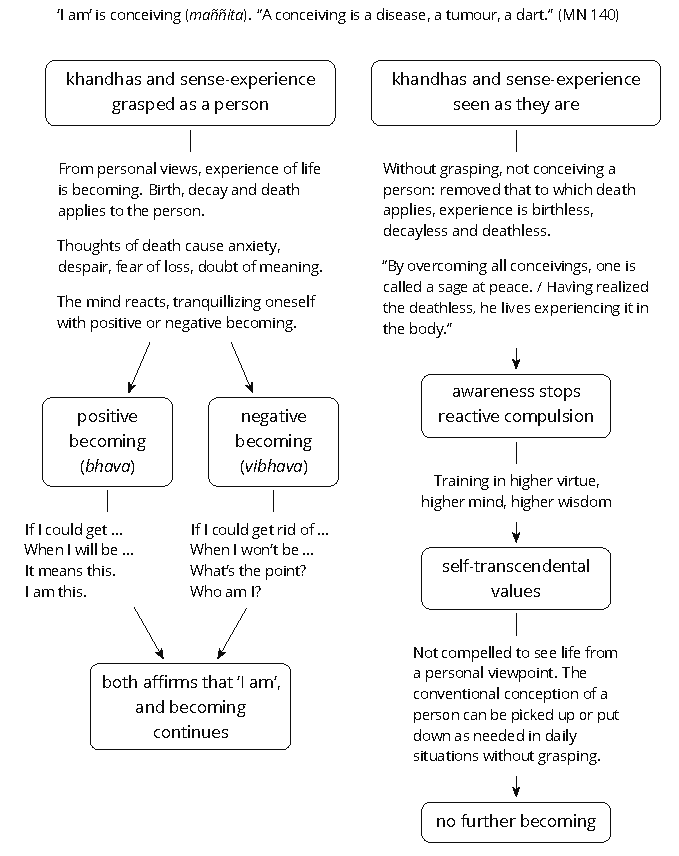
\includegraphics[width=\linewidth]{./manuscript/tex/diagrams/experience-becoming-deathless.pdf}
\end{figure}

{\noindent\footnotesize
See also: Chapter 10, Birth, Decay and Death in The Buddha's Teaching: It's Essential\\ Meaning by R. G. de S. Wettimuny
\par}

\clearpage
\normalpagelayout

\section{New Eyes}

\keywords{turning toward experience, intellectual knowledge, watching the senses}

\noindent We can turn a compulsive tendency into meditation practice by
asking, `How can I understand this experience?' This question directs us
to the noble attitude towards suffering described in the Four Noble
Truths: `Suffering should be understood.' Discard the opinions which
present themselves as answers, and keep returning to this open attitude
of knowing the present.

Both joy and sorrow are natural processes, but if we don't understand
them, we see one as a reward and the other as a punishment. Life never
seems to be fair and it always seems to be out of our control.

To open up our attitude for contemplation, we can at least imagine the
possibility that there is something here we can learn. A turning point
occurs when we are able to let go of being sure about our opinions and
can stop to investigate the experience itself.

Consider how narrow our attitude is when we start with the thought,
`I've seen this, I know this'. Perhaps this is true, but I notice that
when I try to use that intellectual knowledge to solve a problem, my
attention merely revolves around memories, thoughts and opinions. While
I am caught up in the past, the present experience escapes my attention.

The instruction of the Buddha is to establish a careful intention to
meditate, and to put aside the matters of the world.

\clearpage

\begin{quote}
There is the case where a monk remains focused \ldots{} ardent, alert,
and mindful -- subduing greed and distress with reference to the world.

\bigskip

\quoteRef{%

\href{https://suttacentral.net/mn10}{MN 10}, Mindfulness Meditation

}
\end{quote}

The thoughts and opinions don't become `our knowledge', but we can
understand the process of their arising and ceasing. `\emph{What} is it
that I am doing? \emph{How} am I doing it?' Letting go of our fixed
positions becomes the way forward; we discover it by seeing with new
eyes.\footnote{`The real voyage of discovery consists not in seeking new
  landscapes, but in having new eyes.' (Marcel Proust)} Life may still
not be fair or entirely under our control, but now we are familiar with
a practice which makes the difference between knowing mental states and
having a mental breakdown.

The fundamental principle is that watching the mind develops the mind. A
wakeful awareness unbinds the compulsive tendencies. We cannot know what
is going to happen tomorrow, but there will be change. The word `Buddha'
means `one who knows, one who is awake'. The source of contentment in
activity is that we continue to trust and practice living in this
wakeful awareness.

\chapter{Silence}

\section{Signal}

\keywords{relation with our surroundings}

Two of us are walking down a path leading to the entrance of the
monastery. We are talking about one thing or another, but as we enter,
we notice the silence and our conversation stops. The Dhamma hall is
beyond the next door, and we don't want to disturb anyone who might be
meditating inside. We close the door quietly behind us. We are going
somewhere else in the building, but the significance of the Dhamma hall
is above that mundane task.

The silence of listening creates an implied relation with our
surroundings. In the previous case with the person who could be sitting
in the Dhamma hall, but even if we could see that there is nobody there,
we would still lower our voices or stay silent. When we enter, the
silence serves as a signal to pay attention. We give space for the
values beyond ourselves represented by the Dhamma hall dedicated to the
truths of the heart and mind.

In this context, silence is a signal which directs us to remember that
which is beyond the worldly values. When we enter a church, monastery or
other sacred spaces, we look beyond noisy worldly affairs and beyond our
usual preoccupation with ourselves.

We have enough experience of noisy chatter to know that profound
comprehension is not found there. So we fall silent to give our
attention to listening, to be a part of the understanding we cannot
express in words. We move in silence, we listen in silence, carefully
keeping ourselves out of the way, so that we may hear the message of the
place and let the activity speak for itself. This silence is a presence,
not isolating, but including the space and the other beings who live
there. In the words of David Whyte,\footnote{\href{https://www.goodreads.com/quotes/10119971-the-winter-of-listening-no-one-but-me-by-the}{The
  Winter of Listening by David Whyte}}

\begin{quote}
You can belong\\
to everything\\
simply by listening.
\end{quote}

\section{Valuable}

\keywords{paying attention, serenity in silence}

Silence also expresses how much we value what we are doing. Being silent
and maintaining attention is an expression of alertness and respect for
that activity. This is both an inward and outward signal: Others see
that whatever we are doing, it requires silence. We also see ourselves
being silent, voluntarily restraining our impact on ourselves and on our
surroundings, which communicates that where we are and what we are doing
has more significance than chattering about ourselves.

Calmness, understanding and silence are closely connected. We stop
speaking and pay careful attention to investigate and understand a
phenomena. After this verbal silence, the mind continues, `Why? Why?',
but when the penny drops at the `Aha!' moment, the mind also stops
chattering and we are silent, feeling glad for the understanding. In
that content and serene mood, we stay silent, for the moment nothing
further is required.

\begin{quote}
On hearing true teachings\\
the hearts of those who are receptive\\
become serene,\\
like a lake, deep, clear and still.

\bigskip

\quoteRef{%

Dhp 82.\footnote{\href{https://forestsangha.org/teachings/books/a-dhammapada-for-contemplation?language=English}{A
  Dhammapada for Contemplation by Ajahn Munindo (2017,
  forestsangha.org)}}

}
\end{quote}

\keywords{lying down meditation method}

Stillness is most characteristic in the lying down meditation posture.
In this posture the muscles of the body are completely relaxed, which
creates a sense of ease and comfort, although one has to take care and
avoid falling asleep. When you are physically tired, this posture is not
recommended for meditation, but rather the sitting, walking or standing
postures, which raise the body's energy level by the physical effort.

Establish a clear intention to be wakeful. Before lying down, it sets
the right attitude and separates us from the daily activities, if we
first bow to a Buddha shrine, and softly recite a short chant.

\clearpage
\thispagestyle{empty}\mbox{}
\photoFullBleedPlaceholder{TODO: Illustration of lying down meditation.}
\clearpage

A yoga mat or soft carpet is useful to avoid getting sore when lying on
the floor. If you feel the breathing becoming obstructed as the head
inclines backward, use a small, firm pillow or a folded towel to prop up
your head. Lying down in a bed could be too soft, and it reminds the
body about sleeping. Let the hands rest at the side of the body. If you
place them on the belly or the chest, the rising and falling movement
can be distracting. Pull up the knees, so that the feet can be flat on
the mat. This avoids tension in the joints and helps to maintain
alertness.

Maintain this posture while relaxing the muscles in the body and
cultivate physical stillness. Direct attention inward and use the
sensation of breathing as your meditation. Experiment with the breath,
use it to brighten the mind and maintain clear comprehension. If the
mind drifts into dull greyness, drowsiness will follow. Setting a timer
could be appropriate, either to signal the end of the session, or as a
periodic reminder to remain alert.

\keywords{noise exposure, available cognitive capacity}

Speaking of the advantages of silence is not to say that sound cannot be
pleasant. Music clearly has therapeutic effects, and helps to relax an
agitated mind. It can be \emph{very good music} (in our opinion), but
how many times in a row can you listen to it? One single thing over and
over, it turns from pleasant to painful in a short time. Have you
listened to music for hours, thinking, `I like this music', but still
feeling relieved when you turned it off? `Good song, but I've been
missing this silence.'

Sounds are input signals which stimulate the nervous system, it can feel
good for a while, but it is still a continuous stimulation. Noisy
environments degrade attention and intelligence, you can probably
remember how hard it is to think clearly when there is a construction
site at your neighbour's property. Apart from personal experience,
medical studies have also measured how `mental workload and visual /
auditory attention is significantly reduced'\footnote{\href{https://www.ncbi.nlm.nih.gov/pmc/articles/PMC6901841/}{The
  Effect of Noise Exposure on Cognitive Performance and Brain Activity
  Patterns (2019, www.ncbi.nlm.nih.gov)}} when being exposed to noise.

Mobile phones don't even have to make a noise to cause `brain drain':
another study found that `the mere presence of one's own smartphone
reduces available cognitive capacity'.\footnote{\href{https://www.journals.uchicago.edu/doi/10.1086/691462}{Brain
  Drain: The Mere Presence of One's Own Smartphone Reduces Available
  Cognitive Capacity (2017, www.journals.uchicago.edu)}} It is not
surprising that traditional insight meditation retreats try to setup a
silent environment and ask participant to not bring their mobile phones
to the meditation hall, or leave them in a locked place for the entire
retreat. Give that nervous system a break and let it settle, don't let
it be like the crow in Santoka's haiku,\footnote{\href{https://www.goodreads.com/book/show/931086.Grass_and_Tree_Cairn}{Grass
  and Tree Cairn, Taneda Santoka}}

\begin{quote}
Cawing a crow,\\
flapping a crow,\\
with no place to settle down.
\end{quote}

\clearpage

\section{Chanting}

\keywords{setting a clear intention, wholesome thoughts}

At the monastery, we practise chanting before or after the daily group
meditations. First, when we arrive individually to the Dhamma hall, we
bow three times in silence toward the Buddha shrine. The senior monk
rings a small bell to signal the start of the chanting. We wait in
silence while he lights the candles and incense on the shrine, and we
bow again. During the bowing, there is always silence.

We begin the chanting together, synchronizing our voices: too soft can't
be heard, too loud is harsh and being out of tune, separates from the
harmony. (A good guideline is that if you don't hear your own voice, you
are chanting too softly, and if you can only hear yourself, you are too
loud.) The text of the chants are recollections of the Buddha and the
teachings, this is a practice of directing the mind toward thinking
wholesome thoughts. This ordered, symbolic ceremony uses a rhythm of
speech and action as a skilful tool to clear the mind before the silence
of meditation.

The exact routine varies between monasteries. The morning meditation at
Sumedhārāma in Portugal starts at 5am, when we start with an hour of
sitting meditation, during which there is no speaking or chanting. When
you enter, there is silence, a shared space for inner reflection for an
hour, until the senior monk rings the bell at the end of the meditation,
which is followed by 15-20 minutes of chanting.

\clearpage

\keywords{boredom, learning about the mind, inner peace, sense-restraint}

`Doesn't it get boring?' From time to time, a school program brings a
whole class of children to meditate in silence (perhaps hoping that they
become more quiet afterward), and they probably do feel bored out of
their skull. They had no interest to be there from the outset, but
children are clever and they tolerate the strange ideas of the adults.

Boredom changes as soon as you look at it. When you come to meditate,
you are interested in learning about yourself and your mind, and looking
at it closer, `boring' becomes rather interesting. `Not much is
happening, just the breathing. Is that a problem for me? \emph{Am I}
creating that problem? Can I stop creating problems for myself? The
breathing has a subtle richness, a pleasant feeling actually.'

When practising mindfulness of breathing, there is a gladness born of
sense restraint. The mind relaxes, and the thinking can be allowed to
stop. We are silently observing experience, there is no need to comment.

Boredom is a combination of factors: the desire for excitement, active
dismissal of the present, and the attitude that we already know, there
is nothing new here. Is it not intrinsic quality of the situation, but
rather a habit of the untrained and restless mind. The Buddha compared
it to how an elephant feels when the trainer first restrains him by
tying him to a strong post. The elephant is unfit to train while he
keeps longing to wander in the wilderness as he wishes, but a good
trainer gradually restrains his restlessness until he learns to remain
content.\footnote{\href{https://suttacentral.net/mn125}{MN 125}, The
  Level of the Tamed} In the sutta, Prince Jayasena doesn't even believe
that inner peace is possible through sense-restraint, since he lives in
a palace surrounded by distractions and never experienced with such
peace.

In the meditation hall the door is open, you can stand up and walk out
any time. But you are there because your mind have wandered as you
wished before, but felt that it was ultimately unsatisfactory, and the
untrained mind kept making painful mistakes and trouble. If you walk a
thousand steps in a thousand directions, you just get tired, and angry
why you didn't get anywhere. We pass a threshold when we recognize the
need to be the trainer of our restless mind. We learn what the right
direction is and keep stepping that way.

\begin{quote}
For the mind that is difficult to subdue,\\
flighty, flitting wherever it will,\\
restraint is good,\\
a restrained mind brings happiness.

\bigskip

\quoteRef{%

Dhp 35.\footnote{\href{https://www.ancient-buddhist-texts.net/English-Texts/Dhamma-Verses/03-Mind.htm}{Dhammapada,
  trans. by Ānandajoti Bhikkhu (2017, www.ancient-buddhist-texts.net)}}

}
\end{quote}

\clearpage

\section{Shrine}

\keywords{creating sacred spaces, symbolism of a Buddha shrine}

I didn't always have a Buddha shrine in the room or hut where I stayed
at the monastery. I thought they were part of conforming to
institutional expectations. So I mostly ignored and subtly resented
pictures and statues, because I felt other people expected me to
venerate them, and spitefully I wasn't going to do what (I thought) they
expect. My reaction was like that of school kids: I was clever enough to
tolerate the symbols and arrogant enough to think I already know what
they mean. Believing oneself clever makes one feel superficially
dismissive and bored with everything. It is a self-stupefying
combination, thinking that \emph{I know} closes our mind, so we can't
learn that we don't know. The British psychologist Iain McGilchrist
compares it to being stuck in a labyrinth of mirrors:\footnote{\href{https://www.goodreads.com/book/show/6968772-the-master-and-his-emissary}{The
  Master and His Emissary: The Divided Brain and the Making of the
  Western World by Iain McGilchrist (2009)}} all you can see is what you
tell yourself, and never find a way out.

A small crack must have appeared on those mirrors, because I noticed
that in fact, nobody was making such judgment and expectation of me. I
was creating both sides of the story and I felt consumed over something
I only imagined.

Making a Buddha shrine opens up a small space in the place we live, a
reminder to stop the hurry and make space for awakening. The Buddha
shrine in the meditation hall gives us the same message through silence.
A shrine is a gift for us from ourselves. It is not for answering other
people's expectations, or even for the Buddha. The historical Buddha
passed away 2600 years ago and is beyond expecting or needing anything
from us. Other people have enough to worry about and don't think about
us as much as we assume.

I remember thinking, `Why don't I have space for the Buddha in the place
where I live?' Then I started to cut some wood planks and made a small
shelf for the shrine. Buddha shrines are often quite plain: one or more
Buddha figures, candles, incense and flowers. The Buddha represents
awakened consciousness in the human form. The candles are for wisdom
which makes things visible, as the light in darkness. The incense refers
to a saying of the Buddha about virtue, `the fragrance of virtue
pervades all directions' (Dhp 54).\footnote{Dhammapada verse 54: `The
  fragrance of flowers or sandalwood blows only with the prevailing
  wind, but the fragrance of virtue pervades all directions.' (Trans.
  Ajahn Munindo)} The flowers are a symbol of virtue, happiness and
impermanence. They are like our practice: they bring happiness if we
take good care of them and renew them frequently, while their fading is
a reminder of transience.

I offer these words of reflection with the intention that they may
encourage your practice. The teacher is the Buddha, the source of
illuminating explanations leads back to him. I am grateful that his
teachings have been carried on through the centuries by each generation
to this day. May they help turning the noisy confusion in our mind into
understanding silence.


%\backmatter


%\input{./manuscript/tex/references.tex}

%\cleartorecto
\thispagestyle{plain}

{\fontsize{10}{14}\selectfont%
\setlength{\parindent}{0pt}%
\raggedright\label{copyright-details}%
\setlength{\parskip}{7pt}%

{\centering

{\LARGE\ccbyncnd}

This work is licensed under a Creative Commons\\
Attribution-NonCommercial-NoDerivatives 4.0 International~License.\footnote{%
\href{https://creativecommons.org/licenses/by-nc-nd/4.0/}{https://creativecommons.org/licenses/by-nc-nd/4.0/}}

}

You are free to:

\begin{packeditemize}
\item Share — copy and redistribute the material in any medium or format
\end{packeditemize}

The licensor cannot revoke these freedoms as long as you follow the license terms.

Under the following terms:

\begin{packeditemize}
\item Attribution — You must give appropriate credit, provide a link to the license, and indicate if changes were made. You may do so in any reasonable manner, but not in any way that suggests the licensor endorses you or your use.
\item NonCommercial — You may not use the material for commercial purposes.
\item NoDerivatives — If you remix, transform, or build upon the material, you may not distribute the modified material.
\end{packeditemize}

No additional restrictions — You may not apply legal terms or technological measures that legally restrict others from doing anything the license permits.

Notices:

You do not have to comply with the license for elements of the material in the public domain or where your use is permitted by an applicable exception or limitation.

No warranties are given. The license may not give you all of the permissions necessary for your intended use. For example, other rights such as publicity, privacy, or moral rights may limit how you use the material.

% TODO confirm this notice with The Publisher

\thePublisher\ asserts its moral right to be identified as the author of this book.

\thePublisher\ requests that you attribute ownership of the work to \thePublisher\ on copying, distribution, display or performance of the work.

}


\emptyUntilEven

\end{document}
